
\begin{enumerate}
\item Написать программу на Python, которая реализует бинарное дерево поиска с инкапсуляцией внутренней структуры. Программа должна создавать экземпляры класса TreeNode, которые представляют узлы дерева, и класса SearchTree, который представляет дерево поиска. Класс SearchTree должен содержать методы для добавления, поиска и удаления элементов из дерева, при этом все вспомогательные методы должны быть приватными. Программа также должна создавать дерево поиска, вставлять в него случайные числа и выполнять поиск элементов в дереве.

Инструкции:
\begin{enumerate}
    \item Создайте класс TreeNode с методом \_\_init\_\_, который принимает значение в качестве аргумента и сохраняет его в атрибуте self.data. Атрибуты left и right должны быть инициализированы как None.
    \item Создайте класс SearchTree с методом \_\_init\_\_, который инициализирует корневой узел дерева как None.
    \item Создайте публичный метод add в классе SearchTree, который добавляет значение в дерево. Если корневой узел отсутствует, создайте новый узел с добавляемым значением. В противном случае, вызовите приватный метод \_add\_helper, передав ему корень и значение.
    \item Создайте приватный метод \_add\_helper в классе SearchTree, который рекурсивно добавляет значение в дерево. Если значение меньше или равно значению текущего узла, добавьте его в левое поддерево. Если значение строго больше значения текущего узла, добавьте его в правое поддерево.
    \item Создайте публичный метод locate в классе SearchTree, который ищет значение в дереве. Если дерево пустое, верните None. В противном случае, вызовите приватный метод \_locate\_helper, передав ему корень и искомое значение.
    \item Создайте приватный метод \_locate\_helper в классе SearchTree, который рекурсивно ищет значение в дереве. Если текущий узел равен None или значение текущего узла равно искомому значению, верните текущий узел. В противном случае, рекурсивно вызывайте метод \_locate\_helper для поиска значения в левом поддереве (если искомое значение меньше или равно значению текущего узла) или в правом поддереве (если искомое значение больше).
    \item Создайте экземпляр класса SearchTree и вставьте в него 15 случайных чисел от 1 до 30.
    \item Выполните поиск элементов в дереве и выведите результаты на экран.
\end{enumerate}

Пример использования:
\begin{lstlisting}[language=Python]
tree = SearchTree()
for i in range(15):
    tree.add(random.randint(1, 30))

print("Поиск элементов:")
print(tree.locate(7))   # Обнаружено, возвращен узел (7)
print(tree.locate(25))  # Не обнаружено, возвращено None
print(tree.locate(15))  # Обнаружено, возвращен узел (15)
\end{lstlisting}

\begin{figure}[h]
\centering
\begin{tikzpicture}[level distance=1.5cm,
  level 1/.style={sibling distance=3cm},
  level 2/.style={sibling distance=1.5cm}]
  \node {10}
    child {node {5}
      child {node {2}}
      child {node {8}}
    }
    child {node {15}
      child {node {12}}
      child {node {20}}
    };
\end{tikzpicture}
\caption{Пример бинарного дерева поиска}
\end{figure}

\item Написать программу на Python, которая реализует бинарное дерево поиска с соблюдением принципов инкапсуляции. Программа должна создавать экземпляры класса Vertex, которые представляют узлы дерева, и класса BinaryTree, который представляет дерево поиска. Класс BinaryTree должен содержать методы для вставки, поиска и удаления элементов, при этом все рекурсивные вспомогательные методы должны быть скрыты от внешнего доступа. Программа также должна создавать дерево поиска, вставлять в него случайные числа и выполнять поиск элементов в дереве.

Инструкции:
\begin{enumerate}
    \item Создайте класс Vertex с методом \_\_init\_\_, который принимает значение value и сохраняет его в атрибуте self.key. Атрибуты self.left\_child и self.right\_child должны быть инициализированы как None.
    \item Создайте класс BinaryTree с методом \_\_init\_\_, который инициализирует атрибут self.top как None.
    \item Создайте публичный метод put в классе BinaryTree, который вставляет значение в дерево. Если self.top отсутствует, создайте новый узел с вставляемым значением. В противном случае, вызовите приватный метод \_put\_recursively, передав ему self.top и значение.
    \item Создайте приватный метод \_put\_recursively в классе BinaryTree, который рекурсивно вставляет значение в дерево. Если значение строго меньше значения текущего узла, вставьте его в левое поддерево. Если значение больше или равно значению текущего узла, вставьте его в правое поддерево.
    \item Создайте публичный метод find в классе BinaryTree, который ищет значение в дереве. Если дерево пустое, верните None. В противном случае, вызовите приватный метод \_find\_recursively, передав ему self.top и искомое значение.
    \item Создайте приватный метод \_find\_recursively в классе BinaryTree, который рекурсивно ищет значение в дереве. Если текущий узел равен None или значение текущего узла равно искомому значению, верните текущий узел. В противном случае, рекурсивно вызывайте метод \_find\_recursively для поиска значения в левом поддереве (если искомое значение меньше текущего) или в правом поддереве (если искомое значение больше или равно текущему).
    \item Создайте экземпляр класса BinaryTree и вставьте в него 18 случайных чисел от 5 до 35.
    \item Выполните поиск элементов в дереве и выведите результаты на экран.
\end{enumerate}

Пример использования:
\begin{lstlisting}[language=Python]
bt = BinaryTree()
for i in range(18):
    bt.put(random.randint(5, 35))

print("Поиск элементов:")
print(bt.find(10))  # Обнаружено, возвращен узел (10)
print(bt.find(40))  # Не обнаружено, возвращено None
print(bt.find(22))  # Обнаружено, возвращен узел (22)
\end{lstlisting}

\begin{figure}[h]
\centering
\begin{tikzpicture}[level distance=1.5cm,
  level 1/.style={sibling distance=3cm},
  level 2/.style={sibling distance=1.5cm}]
  \node {18}
    child {node {9}
      child {node {4}}
      child {node {14}}
    }
    child {node {25}
      child {node {21}}
      child {node {30}}
    };
\end{tikzpicture}
\caption{Пример бинарного дерева поиска}
\end{figure}

\item Написать программу на Python, которая реализует бинарное дерево поиска с инкапсуляцией внутренней логики. Программа должна создавать экземпляры класса BNode, которые представляют узлы дерева, и класса BSTree, который представляет дерево поиска. Класс BSTree должен содержать методы для вставки, поиска и удаления элементов, при этом все рекурсивные функции должны быть приватными. Программа также должна создавать дерево поиска, вставлять в него случайные числа и выполнять поиск элементов в дереве.

Инструкции:
\begin{enumerate}
    \item Создайте класс BNode с методом \_\_init\_\_, который принимает параметр item и сохраняет его в атрибуте self.element. Атрибуты self.left\_branch и self.right\_branch должны быть инициализированы как None.
    \item Создайте класс BSTree с методом \_\_init\_\_, который инициализирует атрибут self.root\_node как None.
    \item Создайте публичный метод insert\_value в классе BSTree, который вставляет значение в дерево. Если self.root\_node отсутствует, создайте новый узел с вставляемым значением. В противном случае, вызовите приватный метод \_recursive\_insert, передав ему self.root\_node и значение.
    \item Создайте приватный метод \_recursive\_insert в классе BSTree, который рекурсивно вставляет значение в дерево. Если значение меньше или равно значению текущего узла, вставьте его в левое поддерево. Если значение строго больше значения текущего узла, вставьте его в правое поддерево.
    \item Создайте публичный метод retrieve в классе BSTree, который ищет значение в дереве. Если дерево пустое, верните None. В противном случае, вызовите приватный метод \_recursive\_retrieve, передав ему self.root\_node и искомое значение.
    \item Создайте приватный метод \_recursive\_retrieve в классе BSTree, который рекурсивно ищет значение в дереве. Если текущий узел равен None или значение текущего узла равно искомому значению, верните текущий узел. В противном случае, рекурсивно вызывайте метод \_recursive\_retrieve для поиска значения в левом поддереве (если искомое значение меньше или равно текущему) или в правом поддереве (если искомое значение больше).
    \item Создайте экземпляр класса BSTree и вставьте в него 20 случайных чисел от 1 до 40.
    \item Выполните поиск элементов в дереве и выведите результаты на экран.
\end{enumerate}

Пример использования:
\begin{lstlisting}[language=Python]
bst = BSTree()
for i in range(20):
    bst.insert_value(random.randint(1, 40))

print("Поиск элементов:")
print(bst.retrieve(12))  # Обнаружено, возвращен узел (12)
print(bst.retrieve(50))  # Не обнаружено, возвращено None
print(bst.retrieve(33))  # Обнаружено, возвращен узел (33)
\end{lstlisting}

\begin{figure}[h]
\centering
\begin{tikzpicture}[level distance=1.5cm,
  level 1/.style={sibling distance=3cm},
  level 2/.style={sibling distance=1.5cm}]
  \node {20}
    child {node {10}
      child {node {5}}
      child {node {15}}
    }
    child {node {30}
      child {node {25}}
      child {node {35}}
    };
\end{tikzpicture}
\caption{Пример бинарного дерева поиска}
\end{figure}

\item Написать программу на Python, которая реализует бинарное дерево поиска с инкапсуляцией. Программа должна создавать экземпляры класса ElementNode, которые представляют узлы дерева, и класса OrderedTree, который представляет дерево поиска. Класс OrderedTree должен содержать методы для вставки, поиска и удаления элементов, при этом все вспомогательные методы должны быть приватными. Программа также должна создавать дерево поиска, вставлять в него случайные числа и выполнять поиск элементов в дереве.

Инструкции:
\begin{enumerate}
    \item Создайте класс ElementNode с методом \_\_init\_\_, который принимает параметр content и сохраняет его в атрибуте self.payload. Атрибуты self.left и self.right должны быть инициализированы как None.
    \item Создайте класс OrderedTree с методом \_\_init\_\_, который инициализирует атрибут self.head как None.
    \item Создайте публичный метод store в классе OrderedTree, который вставляет значение в дерево. Если self.head отсутствует, создайте новый узел с вставляемым значением. В противном случае, вызовите приватный метод \_store\_recursive, передав ему self.head и значение.
    \item Создайте приватный метод \_store\_recursive в классе OrderedTree, который рекурсивно вставляет значение в дерево. Если значение строго меньше значения текущего узла, вставьте его в левое поддерево. Если значение больше или равно значению текущего узла, вставьте его в правое поддерево.
    \item Создайте публичный метод query в классе OrderedTree, который ищет значение в дереве. Если дерево пустое, верните None. В противном случае, вызовите приватный метод \_query\_recursive, передав ему self.head и искомое значение.
    \item Создайте приватный метод \_query\_recursive в классе OrderedTree, который рекурсивно ищет значение в дереве. Если текущий узел равен None или значение текущего узла равно искомому значению, верните текущий узел. В противном случае, рекурсивно вызывайте метод \_query\_recursive для поиска значения в левом поддереве (если искомое значение меньше текущего) или в правом поддереве (если искомое значение больше или равно текущему).
    \item Создайте экземпляр класса OrderedTree и вставьте в него 17 случайных чисел от 3 до 33.
    \item Выполните поиск элементов в дереве и выведите результаты на экран.
\end{enumerate}

Пример использования:
\begin{lstlisting}[language=Python]
ot = OrderedTree()
for i in range(17):
    ot.store(random.randint(3, 33))

print("Поиск элементов:")
print(ot.query(8))   # Обнаружено, возвращен узел (8)
print(ot.query(45))  # Не обнаружено, возвращено None
print(ot.query(27))  # Обнаружено, возвращен узел (27)
\end{lstlisting}

\begin{figure}[h]
\centering
\begin{tikzpicture}[level distance=1.5cm,
  level 1/.style={sibling distance=3cm},
  level 2/.style={sibling distance=1.5cm}]
  \node {17}
    child {node {8}
      child {node {3}}
      child {node {12}}
    }
    child {node {27}
      child {node {22}}
      child {node {32}}
    };
\end{tikzpicture}
\caption{Пример бинарного дерева поиска}
\end{figure}

\item Написать программу на Python, которая реализует бинарное дерево поиска с инкапсуляцией внутренней структуры. Программа должна создавать экземпляры класса DataNode, которые представляют узлы дерева, и класса SortedTree, который представляет дерево поиска. Класс SortedTree должен содержать методы для вставки, поиска и удаления элементов, при этом все рекурсивные методы должны быть скрыты. Программа также должна создавать дерево поиска, вставлять в него случайные числа и выполнять поиск элементов в дереве.

Инструкции:
\begin{enumerate}
    \item Создайте класс DataNode с методом \_\_init\_\_, который принимает параметр val и сохраняет его в атрибуте self.entry. Атрибуты self.left и self.right должны быть инициализированы как None.
    \item Создайте класс SortedTree с методом \_\_init\_\_, который инициализирует атрибут self.first\_node как None.
    \item Создайте публичный метод enqueue в классе SortedTree, который вставляет значение в дерево. Если self.first\_node отсутствует, создайте новый узел с вставляемым значением. В противном случае, вызовите приватный метод \_enqueue\_helper, передав ему self.first\_node и значение.
    \item Создайте приватный метод \_enqueue\_helper в классе SortedTree, который рекурсивно вставляет значение в дерево. Если значение меньше или равно значению текущего узла, вставьте его в левое поддерево. Если значение строго больше значения текущего узла, вставьте его в правое поддерево.
    \item Создайте публичный метод lookup в классе SortedTree, который ищет значение в дереве. Если дерево пустое, верните None. В противном случае, вызовите приватный метод \_lookup\_helper, передав ему self.first\_node и искомое значение.
    \item Создайте приватный метод \_lookup\_helper в классе SortedTree, который рекурсивно ищет значение в дереве. Если текущий узел равен None или значение текущего узла равно искомому значению, верните текущий узел. В противном случае, рекурсивно вызывайте метод \_lookup\_helper для поиска значения в левом поддереве (если искомое значение меньше или равно текущему) или в правом поддереве (если искомое значение больше).
    \item Создайте экземпляр класса SortedTree и вставьте в него 16 случайных чисел от 2 до 28.
    \item Выполните поиск элементов в дереве и выведите результаты на экран.
\end{enumerate}

Пример использования:
\begin{lstlisting}[language=Python]
st = SortedTree()
for i in range(16):
    st.enqueue(random.randint(2, 28))

print("Поиск элементов:")
print(st.lookup(6))   # Обнаружено, возвращен узел (6)
print(st.lookup(35))  # Не обнаружено, возвращено None
print(st.lookup(19))  # Обнаружено, возвращен узел (19)
\end{lstlisting}

\begin{figure}[h]
\centering
\begin{tikzpicture}[level distance=1.5cm,
  level 1/.style={sibling distance=3cm},
  level 2/.style={sibling distance=1.5cm}]
  \node {14}
    child {node {6}
      child {node {2}}
      child {node {10}}
    }
    child {node {22}
      child {node {18}}
      child {node {26}}
    };
\end{tikzpicture}
\caption{Пример бинарного дерева поиска}
\end{figure}

\item Написать программу на Python, которая реализует бинарное дерево поиска с инкапсуляцией. Программа должна создавать экземпляры класса BinNode, которые представляют узлы дерева, и класса LookupTree, который представляет дерево поиска. Класс LookupTree должен содержать методы для вставки, поиска и удаления элементов, при этом все вспомогательные методы должны быть приватными. Программа также должна создавать дерево поиска, вставлять в него случайные числа и выполнять поиск элементов в дереве.

Инструкции:
\begin{enumerate}
    \item Создайте класс BinNode с методом \_\_init\_\_, который принимает параметр num и сохраняет его в атрибуте self.number. Атрибуты self.left и self.right должны быть инициализированы как None.
    \item Создайте класс LookupTree с методом \_\_init\_\_, который инициализирует атрибут self.initial\_node как None.
    \item Создайте публичный метод add\_entry в классе LookupTree, который вставляет значение в дерево. Если self.initial\_node отсутствует, создайте новый узел с вставляемым значением. В противном случае, вызовите приватный метод \_add\_entry\_rec, передав ему self.initial\_node и значение.
    \item Создайте приватный метод \_add\_entry\_rec в классе LookupTree, который рекурсивно вставляет значение в дерево. Если значение строго меньше значения текущего узла, вставьте его в левое поддерево. Если значение больше или равно значению текущего узла, вставьте его в правое поддерево.
    \item Создайте публичный метод fetch в классе LookupTree, который ищет значение в дереве. Если дерево пустое, верните None. В противном случае, вызовите приватный метод \_fetch\_rec, передав ему self.initial\_node и искомое значение.
    \item Создайте приватный метод \_fetch\_rec в классе LookupTree, который рекурсивно ищет значение в дереве. Если текущий узел равен None или значение текущего узла равно искомому значению, верните текущий узел. В противном случае, рекурсивно вызывайте метод \_fetch\_rec для поиска значения в левом поддереве (если искомое значение меньше текущего) или в правом поддереве (если искомое значение больше или равно текущему).
    \item Создайте экземпляр класса LookupTree и вставьте в него 19 случайных чисел от 4 до 34.
    \item Выполните поиск элементов в дереве и выведите результаты на экран.
\end{enumerate}

Пример использования:
\begin{lstlisting}[language=Python]
lt = LookupTree()
for i in range(19):
    lt.add_entry(random.randint(4, 34))

print("Поиск элементов:")
print(lt.fetch(9))   # Обнаружено, возвращен узел (9)
print(lt.fetch(40))  # Не обнаружено, возвращено None
print(lt.fetch(24))  # Обнаружено, возвращен узел (24)
\end{lstlisting}

\begin{figure}[h]
\centering
\begin{tikzpicture}[level distance=1.5cm,
  level 1/.style={sibling distance=3cm},
  level 2/.style={sibling distance=1.5cm}]
  \node {19}
    child {node {9}
      child {node {4}}
      child {node {14}}
    }
    child {node {29}
      child {node {24}}
      child {node {34}}
    };
\end{tikzpicture}
\caption{Пример бинарного дерева поиска}
\end{figure}

\item Написать программу на Python, которая реализует бинарное дерево поиска с инкапсуляцией. Программа должна создавать экземпляры класса NodeItem, которые представляют узлы дерева, и класса BinaryTreeSearch, который представляет дерево поиска. Класс BinaryTreeSearch должен содержать методы для вставки, поиска и удаления элементов, при этом все рекурсивные методы должны быть приватными. Программа также должна создавать дерево поиска, вставлять в него случайные числа и выполнять поиск элементов в дереве.

Инструкции:
\begin{enumerate}
    \item Создайте класс NodeItem с методом \_\_init\_\_, который принимает параметр item\_value и сохраняет его в атрибуте self.val. Атрибуты self.left и self.right должны быть инициализированы как None.
    \item Создайте класс BinaryTreeSearch с методом \_\_init\_\_, который инициализирует атрибут self.start\_node как None.
    \item Создайте публичный метод insert\_item в классе BinaryTreeSearch, который вставляет значение в дерево. Если self.start\_node отсутствует, создайте новый узел с вставляемым значением. В противном случае, вызовите приватный метод \_insert\_item\_helper, передав ему self.start\_node и значение.
    \item Создайте приватный метод \_insert\_item\_helper в классе BinaryTreeSearch, который рекурсивно вставляет значение в дерево. Если значение меньше или равно значению текущего узла, вставьте его в левое поддерево. Если значение строго больше значения текущего узла, вставьте его в правое поддерево.
    \item Создайте публичный метод find\_item в классе BinaryTreeSearch, который ищет значение в дереве. Если дерево пустое, верните None. В противном случае, вызовите приватный метод \_find\_item\_helper, передав ему self.start\_node и искомое значение.
    \item Создайте приватный метод \_find\_item\_helper в классе BinaryTreeSearch, который рекурсивно ищет значение в дереве. Если текущий узел равен None или значение текущего узла равно искомому значению, верните текущий узел. В противном случае, рекурсивно вызывайте метод \_find\_item\_helper для поиска значения в левом поддереве (если искомое значение меньше или равно текущему) или в правом поддереве (если искомое значение больше).
    \item Создайте экземпляр класса BinaryTreeSearch и вставьте в него 21 случайное число от 1 до 38.
    \item Выполните поиск элементов в дереве и выведите результаты на экран.
\end{enumerate}

Пример использования:
\begin{lstlisting}[language=Python]
bts = BinaryTreeSearch()
for i in range(21):
    bts.insert_item(random.randint(1, 38))

print("Поиск элементов:")
print(bts.find_item(11))  # Обнаружено, возвращен узел (11)
print(bts.find_item(50))  # Не обнаружено, возвращено None
print(bts.find_item(29))  # Обнаружено, возвращен узел (29)
\end{lstlisting}

\begin{figure}[h]
\centering
\begin{tikzpicture}[level distance=1.5cm,
  level 1/.style={sibling distance=3cm},
  level 2/.style={sibling distance=1.5cm}]
  \node {21}
    child {node {11}
      child {node {5}}
      child {node {16}}
    }
    child {node {31}
      child {node {26}}
      child {node {36}}
    };
\end{tikzpicture}
\caption{Пример бинарного дерева поиска}
\end{figure}

\item Написать программу на Python, которая реализует бинарное дерево поиска с инкапсуляцией. Программа должна создавать экземпляры класса TreeVertex, которые представляют узлы дерева, и класса SearchBinTree, который представляет дерево поиска. Класс SearchBinTree должен содержать методы для вставки, поиска и удаления элементов, при этом все вспомогательные методы должны быть приватными. Программа также должна создавать дерево поиска, вставлять в него случайные числа и выполнять поиск элементов в дереве.

Инструкции:
\begin{enumerate}
    \item Создайте класс TreeVertex с методом \_\_init\_\_, который принимает параметр vertex\_data и сохраняет его в атрибуте self.info. Атрибуты self.left и self.right должны быть инициализированы как None.
    \item Создайте класс SearchBinTree с методом \_\_init\_\_, который инициализирует атрибут self.root\_vertex как None.
    \item Создайте публичный метод insert\_data в классе SearchBinTree, который вставляет значение в дерево. Если self.root\_vertex отсутствует, создайте новый узел с вставляемым значением. В противном случае, вызовите приватный метод \_insert\_data\_rec, передав ему self.root\_vertex и значение.
    \item Создайте приватный метод \_insert\_data\_rec в классе SearchBinTree, который рекурсивно вставляет значение в дерево. Если значение строго меньше значения текущего узла, вставьте его в левое поддерево. Если значение больше или равно значению текущего узла, вставьте его в правое поддерево.
    \item Создайте публичный метод search\_data в классе SearchBinTree, который ищет значение в дереве. Если дерево пустое, верните None. В противном случае, вызовите приватный метод \_search\_data\_rec, передав ему self.root\_vertex и искомое значение.
    \item Создайте приватный метод \_search\_data\_rec в классе SearchBinTree, который рекурсивно ищет значение в дереве. Если текущий узел равен None или значение текущего узла равно искомому значению, верните текущий узел. В противном случае, рекурсивно вызывайте метод \_search\_data\_rec для поиска значения в левом поддереве (если искомое значение меньше текущего) или в правом поддереве (если искомое значение больше или равно текущему).
    \item Создайте экземпляр класса SearchBinTree и вставьте в него 14 случайных чисел от 6 до 36.
    \item Выполните поиск элементов в дереве и выведите результаты на экран.
\end{enumerate}

Пример использования:
\begin{lstlisting}[language=Python]
sbt = SearchBinTree()
for i in range(14):
    sbt.insert_data(random.randint(6, 36))

print("Поиск элементов:")
print(sbt.search_data(13))  # Обнаружено, возвращен узел (13)
print(sbt.search_data(42))  # Не обнаружено, возвращено None
print(sbt.search_data(28))  # Обнаружено, возвращен узел (28)
\end{lstlisting}

\begin{figure}[h]
\centering
\begin{tikzpicture}[level distance=1.5cm,
  level 1/.style={sibling distance=3cm},
  level 2/.style={sibling distance=1.5cm}]
  \node {23}
    child {node {13}
      child {node {8}}
      child {node {18}}
    }
    child {node {33}
      child {node {28}}
      child {node {38}}
    };
\end{tikzpicture}
\caption{Пример бинарного дерева поиска}
\end{figure}

\item Написать программу на Python, которая реализует бинарное дерево поиска с инкапсуляцией. Программа должна создавать экземпляры класса BranchNode, которые представляют узлы дерева, и класса BinaryTreeLookup, который представляет дерево поиска. Класс BinaryTreeLookup должен содержать методы для вставки, поиска и удаления элементов, при этом все рекурсивные методы должны быть приватными. Программа также должна создавать дерево поиска, вставлять в него случайные числа и выполнять поиск элементов в дереве.

Инструкции:
\begin{enumerate}
    \item Создайте класс BranchNode с методом \_\_init\_\_, который принимает параметр node\_val и сохраняет его в атрибуте self.data\_point. Атрибуты self.left\_link и self.right\_link должны быть инициализированы как None.
    \item Создайте класс BinaryTreeLookup с методом \_\_init\_\_, который инициализирует атрибут self.base\_node как None.
    \item Создайте публичный метод add\_point в классе BinaryTreeLookup, который вставляет значение в дерево. Если self.base\_node отсутствует, создайте новый узел с вставляемым значением. В противном случае, вызовите приватный метод \_add\_point\_recursive, передав ему self.base\_node и значение.
    \item Создайте приватный метод \_add\_point\_recursive в классе BinaryTreeLookup, который рекурсивно вставляет значение в дерево. Если значение меньше или равно значению текущего узла, вставьте его в левое поддерево. Если значение строго больше значения текущего узла, вставьте его в правое поддерево.
    \item Создайте публичный метод locate\_point в классе BinaryTreeLookup, который ищет значение в дереве. Если дерево пустое, верните None. В противном случае, вызовите приватный метод \_locate\_point\_recursive, передав ему self.base\_node и искомое значение.
    \item Создайте приватный метод \_locate\_point\_recursive в классе BinaryTreeLookup, который рекурсивно ищет значение в дереве. Если текущий узел равен None или значение текущего узла равно искомому значению, верните текущий узел. В противном случае, рекурсивно вызывайте метод \_locate\_point\_recursive для поиска значения в левом поддереве (если искомое значение меньше или равно текущему) или в правом поддереве (если искомое значение больше).
    \item Создайте экземпляр класса BinaryTreeLookup и вставьте в него 13 случайных чисел от 7 до 37.
    \item Выполните поиск элементов в дереве и выведите результаты на экран.
\end{enumerate}

Пример использования:
\begin{lstlisting}[language=Python]
btl = BinaryTreeLookup()
for i in range(13):
    btl.add_point(random.randint(7, 37))

print("Поиск элементов:")
print(btl.locate_point(14))  # Обнаружено, возвращен узел (14)
print(btl.locate_point(45))  # Не обнаружено, возвращено None
print(btl.locate_point(27))  # Обнаружено, возвращен узел (27)
\end{lstlisting}

\begin{figure}[h]
\centering
\begin{tikzpicture}[level distance=1.5cm,
  level 1/.style={sibling distance=3cm},
  level 2/.style={sibling distance=1.5cm}]
  \node {24}
    child {node {14}
      child {node {9}}
      child {node {19}}
    }
    child {node {34}
      child {node {29}}
      child {node {39}}
    };
\end{tikzpicture}
\caption{Пример бинарного дерева поиска}
\end{figure}

\item Написать программу на Python, которая реализует бинарное дерево поиска с инкапсуляцией. Программа должна создавать экземпляры класса TreeNodeStruct, которые представляют узлы дерева, и класса BinSearchStructure, который представляет дерево поиска. Класс BinSearchStructure должен содержать методы для вставки, поиска и удаления элементов, при этом все вспомогательные методы должны быть приватными. Программа также должна создавать дерево поиска, вставлять в него случайные числа и выполнять поиск элементов в дереве.

Инструкции:
\begin{enumerate}
    \item Создайте класс TreeNodeStruct с методом \_\_init\_\_, который принимает параметр struct\_value и сохраняет его в атрибуте self.node\_value. Атрибуты self.left\_sub и self.right\_sub должны быть инициализированы как None.
    \item Создайте класс BinSearchStructure с методом \_\_init\_\_, который инициализирует атрибут self.top\_element как None.
    \item Создайте публичный метод insert\_struct в классе BinSearchStructure, который вставляет значение в дерево. Если self.top\_element отсутствует, создайте новый узел с вставляемым значением. В противном случае, вызовите приватный метод \_insert\_struct\_helper, передав ему self.top\_element и значение.
    \item Создайте приватный метод \_insert\_struct\_helper в классе BinSearchStructure, который рекурсивно вставляет значение в дерево. Если значение строго меньше значения текущего узла, вставьте его в левое поддерево. Если значение больше или равно значению текущего узла, вставьте его в правое поддерево.
    \item Создайте публичный метод find\_struct в классе BinSearchStructure, который ищет значение в дереве. Если дерево пустое, верните None. В противном случае, вызовите приватный метод \_find\_struct\_helper, передав ему self.top\_element и искомое значение.
    \item Создайте приватный метод \_find\_struct\_helper в классе BinSearchStructure, который рекурсивно ищет значение в дереве. Если текущий узел равен None или значение текущего узла равно искомому значению, верните текущий узел. В противном случае, рекурсивно вызывайте метод \_find\_struct\_helper для поиска значения в левом поддереве (если искомое значение меньше текущего) или в правом поддереве (если искомое значение больше или равно текущему).
    \item Создайте экземпляр класса BinSearchStructure и вставьте в него 22 случайных числа от 2 до 42.
    \item Выполните поиск элементов в дереве и выведите результаты на экран.
\end{enumerate}

Пример использования:
\begin{lstlisting}[language=Python]
bss = BinSearchStructure()
for i in range(22):
    bss.insert_struct(random.randint(2, 42))

print("Поиск элементов:")
print(bss.find_struct(15))  # Обнаружено, возвращен узел (15)
print(bss.find_struct(55))  # Не обнаружено, возвращено None
print(bss.find_struct(35))  # Обнаружено, возвращен узел (35)
\end{lstlisting}

\begin{figure}[h]
\centering
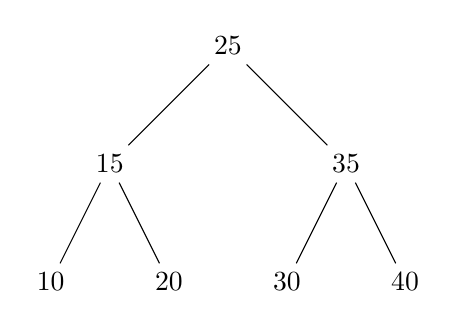
\begin{tikzpicture}[level distance=1.5cm,
  level 1/.style={sibling distance=3cm},
  level 2/.style={sibling distance=1.5cm}]
  \node {25}
    child {node {15}
      child {node {10}}
      child {node {20}}
    }
    child {node {35}
      child {node {30}}
      child {node {40}}
    };
\end{tikzpicture}
\caption{Пример бинарного дерева поиска}
\end{figure}

\item Написать программу на Python, которая реализует бинарное дерево поиска с инкапсуляцией. Программа должна создавать экземпляры класса NodeElement, которые представляют узлы дерева, и класса TreeIndex, который представляет дерево поиска. Класс TreeIndex должен содержать методы для вставки, поиска и удаления элементов, при этом все рекурсивные методы должны быть приватными. Программа также должна создавать дерево поиска, вставлять в него случайные числа и выполнять поиск элементов в дереве.

Инструкции:
\begin{enumerate}
    \item Создайте класс NodeElement с методом \_\_init\_\_, который принимает параметр elem\_value и сохраняет его в атрибуте self.index\_key. Атрибуты self.left и self.right должны быть инициализированы как None.
    \item Создайте класс TreeIndex с методом \_\_init\_\_, который инициализирует атрибут self.root\_elem как None.
    \item Создайте публичный метод add\_key в классе TreeIndex, который вставляет значение в дерево. Если self.root\_elem отсутствует, создайте новый узел с вставляемым значением. В противном случае, вызовите приватный метод \_add\_key\_rec, передав ему self.root\_elem и значение.
    \item Создайте приватный метод \_add\_key\_rec в классе TreeIndex, который рекурсивно вставляет значение в дерево. Если значение меньше или равно значению текущего узла, вставьте его в левое поддерево. Если значение строго больше значения текущего узла, вставьте его в правое поддерево.
    \item Создайте публичный метод get\_key в классе TreeIndex, который ищет значение в дереве. Если дерево пустое, верните None. В противном случае, вызовите приватный метод \_get\_key\_rec, передав ему self.root\_elem и искомое значение.
    \item Создайте приватный метод \_get\_key\_rec в классе TreeIndex, который рекурсивно ищет значение в дереве. Если текущий узел равен None или значение текущего узла равно искомому значению, верните текущий узел. В противном случае, рекурсивно вызывайте метод \_get\_key\_rec для поиска значения в левом поддереве (если искомое значение меньше или равно текущему) или в правом поддереве (если искомое значение больше).
    \item Создайте экземпляр класса TreeIndex и вставьте в него 23 случайных числа от 3 до 43.
    \item Выполните поиск элементов в дереве и выведите результаты на экран.
\end{enumerate}

Пример использования:
\begin{lstlisting}[language=Python]
ti = TreeIndex()
for i in range(23):
    ti.add_key(random.randint(3, 43))

print("Поиск элементов:")
print(ti.get_key(16))  # Обнаружено, возвращен узел (16)
print(ti.get_key(56))  # Не обнаружено, возвращено None
print(ti.get_key(36))  # Обнаружено, возвращен узел (36)
\end{lstlisting}

\begin{figure}[h]
\centering
\begin{tikzpicture}[level distance=1.5cm,
  level 1/.style={sibling distance=3cm},
  level 2/.style={sibling distance=1.5cm}]
  \node {26}
    child {node {16}
      child {node {11}}
      child {node {21}}
    }
    child {node {36}
      child {node {31}}
      child {node {41}}
    };
\end{tikzpicture}
\caption{Пример бинарного дерева поиска}
\end{figure}

\item Написать программу на Python, которая реализует бинарное дерево поиска с инкапсуляцией. Программа должна создавать экземпляры класса BinElement, которые представляют узлы дерева, и класса IndexTree, который представляет дерево поиска. Класс IndexTree должен содержать методы для вставки, поиска и удаления элементов, при этом все вспомогательные методы должны быть приватными. Программа также должна создавать дерево поиска, вставлять в него случайные числа и выполнять поиск элементов в дереве.

Инструкции:
\begin{enumerate}
    \item Создайте класс BinElement с методом \_\_init\_\_, который принимает параметр bin\_val и сохраняет его в атрибуте self.key\_value. Атрибуты self.left\_node и self.right\_node должны быть инициализированы как None.
    \item Создайте класс IndexTree с методом \_\_init\_\_, который инициализирует атрибут self.first\_element как None.
    \item Создайте публичный метод insert\_key в классе IndexTree, который вставляет значение в дерево. Если self.first\_element отсутствует, создайте новый узел с вставляемым значением. В противном случае, вызовите приватный метод \_insert\_key\_helper, передав ему self.first\_element и значение.
    \item Создайте приватный метод \_insert\_key\_helper в классе IndexTree, который рекурсивно вставляет значение в дерево. Если значение строго меньше значения текущего узла, вставьте его в левое поддерево. Если значение больше или равно значению текущего узла, вставьте его в правое поддерево.
    \item Создайте публичный метод search\_key в классе IndexTree, который ищет значение в дереве. Если дерево пустое, верните None. В противном случае, вызовите приватный метод \_search\_key\_helper, передав ему self.first\_element и искомое значение.
    \item Создайте приватный метод \_search\_key\_helper в классе IndexTree, который рекурсивно ищет значение в дереве. Если текущий узел равен None или значение текущего узла равно искомому значению, верните текущий узел. В противном случае, рекурсивно вызывайте метод \_search\_key\_helper для поиска значения в левом поддереве (если искомое значение меньше текущего) или в правом поддереве (если искомое значение больше или равно текущему).
    \item Создайте экземпляр класса IndexTree и вставьте в него 24 случайных числа от 4 до 44.
    \item Выполните поиск элементов в дереве и выведите результаты на экран.
\end{enumerate}

Пример использования:
\begin{lstlisting}[language=Python]
it = IndexTree()
for i in range(24):
    it.insert_key(random.randint(4, 44))

print("Поиск элементов:")
print(it.search_key(17))  # Обнаружено, возвращен узел (17)
print(it.search_key(57))  # Не обнаружено, возвращено None
print(it.search_key(37))  # Обнаружено, возвращен узел (37)
\end{lstlisting}

\begin{figure}[h]
\centering
\begin{tikzpicture}[level distance=1.5cm,
  level 1/.style={sibling distance=3cm},
  level 2/.style={sibling distance=1.5cm}]
  \node {27}
    child {node {17}
      child {node {12}}
      child {node {22}}
    }
    child {node {37}
      child {node {32}}
      child {node {42}}
    };
\end{tikzpicture}
\caption{Пример бинарного дерева поиска}
\end{figure}

\item Написать программу на Python, которая реализует бинарное дерево поиска с инкапсуляцией. Программа должна создавать экземпляры класса SearchNode, которые представляют узлы дерева, и класса BinaryTreeIndex, который представляет дерево поиска. Класс BinaryTreeIndex должен содержать методы для вставки, поиска и удаления элементов, при этом все рекурсивные методы должны быть приватными. Программа также должна создавать дерево поиска, вставлять в него случайные числа и выполнять поиск элементов в дереве.

Инструкции:
\begin{enumerate}
    \item Создайте класс SearchNode с методом \_\_init\_\_, который принимает параметр search\_val и сохраняет его в атрибуте self.node\_key. Атрибуты self.left\_child и self.right\_child должны быть инициализированы как None.
    \item Создайте класс BinaryTreeIndex с методом \_\_init\_\_, который инициализирует атрибут self.initial\_element как None.
    \item Создайте публичный метод add\_node в классе BinaryTreeIndex, который вставляет значение в дерево. Если self.initial\_element отсутствует, создайте новый узел с вставляемым значением. В противном случае, вызовите приватный метод \_add\_node\_recursive, передав ему self.initial\_element и значение.
    \item Создайте приватный метод \_add\_node\_recursive в классе BinaryTreeIndex, который рекурсивно вставляет значение в дерево. Если значение меньше или равно значению текущего узла, вставьте его в левое поддерево. Если значение строго больше значения текущего узла, вставьте его в правое поддерево.
    \item Создайте публичный метод find\_node в классе BinaryTreeIndex, который ищет значение в дереве. Если дерево пустое, верните None. В противном случае, вызовите приватный метод \_find\_node\_recursive, передав ему self.initial\_element и искомое значение.
    \item Создайте приватный метод \_find\_node\_recursive в классе BinaryTreeIndex, который рекурсивно ищет значение в дереве. Если текущий узел равен None или значение текущего узла равно искомому значению, верните текущий узел. В противном случае, рекурсивно вызывайте метод \_find\_node\_recursive для поиска значения в левом поддереве (если искомое значение меньше или равно текущему) или в правом поддереве (если искомое значение больше).
    \item Создайте экземпляр класса BinaryTreeIndex и вставьте в него 25 случайных чисел от 5 до 45.
    \item Выполните поиск элементов в дереве и выведите результаты на экран.
\end{enumerate}

Пример использования:
\begin{lstlisting}[language=Python]
bti = BinaryTreeIndex()
for i in range(25):
    bti.add_node(random.randint(5, 45))

print("Поиск элементов:")
print(bti.find_node(18))  # Обнаружено, возвращен узел (18)
print(bti.find_node(58))  # Не обнаружено, возвращено None
print(bti.find_node(38))  # Обнаружено, возвращен узел (38)
\end{lstlisting}

\begin{figure}[h]
\centering
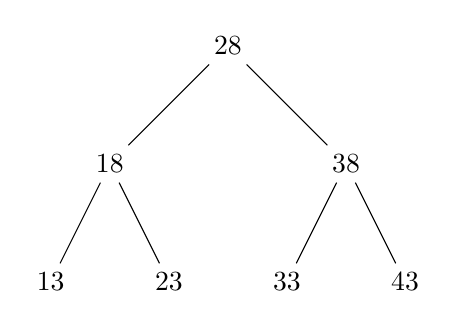
\begin{tikzpicture}[level distance=1.5cm,
  level 1/.style={sibling distance=3cm},
  level 2/.style={sibling distance=1.5cm}]
  \node {28}
    child {node {18}
      child {node {13}}
      child {node {23}}
    }
    child {node {38}
      child {node {33}}
      child {node {43}}
    };
\end{tikzpicture}
\caption{Пример бинарного дерева поиска}
\end{figure}

\item Написать программу на Python, которая реализует бинарное дерево поиска с инкапсуляцией. Программа должна создавать экземпляры класса IndexNode, которые представляют узлы дерева, и класса SearchStructure, который представляет дерево поиска. Класс SearchStructure должен содержать методы для вставки, поиска и удаления элементов, при этом все вспомогательные методы должны быть приватными. Программа также должна создавать дерево поиска, вставлять в него случайные числа и выполнять поиск элементов в дереве.

Инструкции:
\begin{enumerate}
    \item Создайте класс IndexNode с методом \_\_init\_\_, который принимает параметр idx\_value и сохраняет его в атрибуте self.element\_key. Атрибуты self.left\_elem и self.right\_elem должны быть инициализированы как None.
    \item Создайте класс SearchStructure с методом \_\_init\_\_, который инициализирует атрибут self.start\_element как None.
    \item Создайте публичный метод insert\_elem в классе SearchStructure, который вставляет значение в дерево. Если self.start\_element отсутствует, создайте новый узел с вставляемым значением. В противном случае, вызовите приватный метод \_insert\_elem\_rec, передав ему self.start\_element и значение.
    \item Создайте приватный метод \_insert\_elem\_rec в классе SearchStructure, который рекурсивно вставляет значение в дерево. Если значение строго меньше значения текущего узла, вставьте его в левое поддерево. Если значение больше или равно значению текущего узла, вставьте его в правое поддерево.
    \item Создайте публичный метод locate\_elem в классе SearchStructure, который ищет значение в дереве. Если дерево пустое, верните None. В противном случае, вызовите приватный метод \_locate\_elem\_rec, передав ему self.start\_element и искомое значение.
    \item Создайте приватный метод \_locate\_elem\_rec в классе SearchStructure, который рекурсивно ищет значение в дереве. Если текущий узел равен None или значение текущего узла равно искомому значению, верните текущий узел. В противном случае, рекурсивно вызывайте метод \_locate\_elem\_rec для поиска значения в левом поддереве (если искомое значение меньше текущего) или в правом поддереве (если искомое значение больше или равно текущему).
    \item Создайте экземпляр класса SearchStructure и вставьте в него 26 случайных чисел от 6 до 46.
    \item Выполните поиск элементов в дереве и выведите результаты на экран.
\end{enumerate}

Пример использования:
\begin{lstlisting}[language=Python]
ss = SearchStructure()
for i in range(26):
    ss.insert_elem(random.randint(6, 46))

print("Поиск элементов:")
print(ss.locate_elem(19))  # Обнаружено, возвращен узел (19)
print(ss.locate_elem(59))  # Не обнаружено, возвращено None
print(ss.locate_elem(39))  # Обнаружено, возвращен узел (39)
\end{lstlisting}

\begin{figure}[h]
\centering
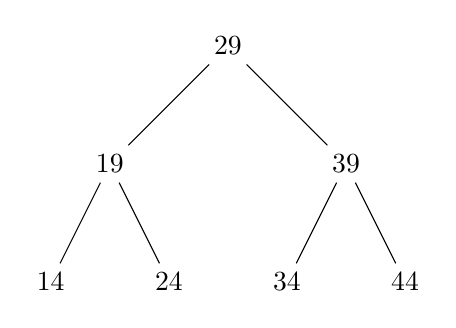
\begin{tikzpicture}[level distance=1.5cm,
  level 1/.style={sibling distance=3cm},
  level 2/.style={sibling distance=1.5cm}]
  \node {29}
    child {node {19}
      child {node {14}}
      child {node {24}}
    }
    child {node {39}
      child {node {34}}
      child {node {44}}
    };
\end{tikzpicture}
\caption{Пример бинарного дерева поиска}
\end{figure}

\item Написать программу на Python, которая реализует бинарное дерево поиска с инкапсуляцией. Программа должна создавать экземпляры класса KeyValueNode, которые представляют узлы дерева, и класса BinaryTreeMap, который представляет дерево поиска. Класс BinaryTreeMap должен содержать методы для вставки, поиска и удаления элементов, при этом все рекурсивные методы должны быть приватными. Программа также должна создавать дерево поиска, вставлять в него случайные числа и выполнять поиск элементов в дереве.

Инструкции:
\begin{enumerate}
    \item Создайте класс KeyValueNode с методом \_\_init\_\_, который принимает параметр key\_val и сохраняет его в атрибуте self.map\_key. Атрибуты self.left\_branch и self.right\_branch должны быть инициализированы как None.
    \item Создайте класс BinaryTreeMap с методом \_\_init\_\_, который инициализирует атрибут self.root\_key как None.
    \item Создайте публичный метод put\_key в классе BinaryTreeMap, который вставляет значение в дерево. Если self.root\_key отсутствует, создайте новый узел с вставляемым значением. В противном случае, вызовите приватный метод \_put\_key\_helper, передав ему self.root\_key и значение.
    \item Создайте приватный метод \_put\_key\_helper в классе BinaryTreeMap, который рекурсивно вставляет значение в дерево. Если значение меньше или равно значению текущего узла, вставьте его в левое поддерево. Если значение строго больше значения текущего узла, вставьте его в правое поддерево.
    \item Создайте публичный метод get\_key в классе BinaryTreeMap, который ищет значение в дереве. Если дерево пустое, верните None. В противном случае, вызовите приватный метод \_get\_key\_helper, передав ему self.root\_key и искомое значение.
    \item Создайте приватный метод \_get\_key\_helper в классе BinaryTreeMap, который рекурсивно ищет значение в дереве. Если текущий узел равен None или значение текущего узла равно искомому значению, верните текущий узел. В противном случае, рекурсивно вызывайте метод \_get\_key\_helper для поиска значения в левом поддереве (если искомое значение меньше или равно текущему) или в правом поддереве (если искомое значение больше).
    \item Создайте экземпляр класса BinaryTreeMap и вставьте в него 27 случайных чисел от 7 до 47.
    \item Выполните поиск элементов в дереве и выведите результаты на экран.
\end{enumerate}

Пример использования:
\begin{lstlisting}[language=Python]
btm = BinaryTreeMap()
for i in range(27):
    btm.put_key(random.randint(7, 47))

print("Поиск элементов:")
print(btm.get_key(20))  # Обнаружено, возвращен узел (20)
print(btm.get_key(60))  # Не обнаружено, возвращено None
print(btm.get_key(40))  # Обнаружено, возвращен узел (40)
\end{lstlisting}

\begin{figure}[h]
\centering
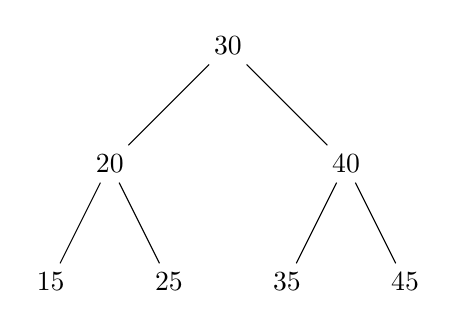
\begin{tikzpicture}[level distance=1.5cm,
  level 1/.style={sibling distance=3cm},
  level 2/.style={sibling distance=1.5cm}]
  \node {30}
    child {node {20}
      child {node {15}}
      child {node {25}}
    }
    child {node {40}
      child {node {35}}
      child {node {45}}
    };
\end{tikzpicture}
\caption{Пример бинарного дерева поиска}
\end{figure}

\item Написать программу на Python, которая реализует бинарное дерево поиска с инкапсуляцией. Программа должна создавать экземпляры класса MapNode, которые представляют узлы дерева, и класса KeyTree, который представляет дерево поиска. Класс KeyTree должен содержать методы для вставки, поиска и удаления элементов, при этом все вспомогательные методы должны быть приватными. Программа также должна создавать дерево поиска, вставлять в него случайные числа и выполнять поиск элементов в дереве.

Инструкции:
\begin{enumerate}
    \item Создайте класс MapNode с методом \_\_init\_\_, который принимает параметр map\_value и сохраняет его в атрибуте self.tree\_key. Атрибуты self.left\_part и self.right\_part должны быть инициализированы как None.
    \item Создайте класс KeyTree с методом \_\_init\_\_, который инициализирует атрибут self.base\_key как None.
    \item Создайте публичный метод insert\_map в классе KeyTree, который вставляет значение в дерево. Если self.base\_key отсутствует, создайте новый узел с вставляемым значением. В противном случае, вызовите приватный метод \_insert\_map\_rec, передав ему self.base\_key и значение.
    \item Создайте приватный метод \_insert\_map\_rec в классе KeyTree, который рекурсивно вставляет значение в дерево. Если значение строго меньше значения текущего узла, вставьте его в левое поддерево. Если значение больше или равно значению текущего узла, вставьте его в правое поддерево.
    \item Создайте публичный метод search\_map в классе KeyTree, который ищет значение в дереве. Если дерево пустое, верните None. В противном случае, вызовите приватный метод \_search\_map\_rec, передав ему self.base\_key и искомое значение.
    \item Создайте приватный метод \_search\_map\_rec в классе KeyTree, который рекурсивно ищет значение в дереве. Если текущий узел равен None или значение текущего узла равно искомому значению, верните текущий узел. В противном случае, рекурсивно вызывайте метод \_search\_map\_rec для поиска значения в левом поддереве (если искомое значение меньше текущего) или в правом поддереве (если искомое значение больше или равно текущему).
    \item Создайте экземпляр класса KeyTree и вставьте в него 28 случайных чисел от 8 до 48.
    \item Выполните поиск элементов в дереве и выведите результаты на экран.
\end{enumerate}

Пример использования:
\begin{lstlisting}[language=Python]
kt = KeyTree()
for i in range(28):
    kt.insert_map(random.randint(8, 48))

print("Поиск элементов:")
print(kt.search_map(21))  # Обнаружено, возвращен узел (21)
print(kt.search_map(61))  # Не обнаружено, возвращено None
print(kt.search_map(41))  # Обнаружено, возвращен узел (41)
\end{lstlisting}

\begin{figure}[h]
\centering
\begin{tikzpicture}[level distance=1.5cm,
  level 1/.style={sibling distance=3cm},
  level 2/.style={sibling distance=1.5cm}]
  \node {31}
    child {node {21}
      child {node {16}}
      child {node {26}}
    }
    child {node {41}
      child {node {36}}
      child {node {46}}
    };
\end{tikzpicture}
\caption{Пример бинарного дерева поиска}
\end{figure}

\item Написать программу на Python, которая реализует бинарное дерево поиска с инкапсуляцией. Программа должна создавать экземпляры класса TreeKeyNode, которые представляют узлы дерева, и класса ValueTree, который представляет дерево поиска. Класс ValueTree должен содержать методы для вставки, поиска и удаления элементов, при этом все рекурсивные методы должны быть приватными. Программа также должна создавать дерево поиска, вставлять в него случайные числа и выполнять поиск элементов в дереве.

Инструкции:
\begin{enumerate}
    \item Создайте класс TreeKeyNode с методом \_\_init\_\_, который принимает параметр tree\_key\_val и сохраняет его в атрибуте self.value\_key. Атрибуты self.left и self.right должны быть инициализированы как None.
    \item Создайте класс ValueTree с методом \_\_init\_\_, который инициализирует атрибут self.first\_key как None.
    \item Создайте публичный метод add\_value в классе ValueTree, который вставляет значение в дерево. Если self.first\_key отсутствует, создайте новый узел с вставляемым значением. В противном случае, вызовите приватный метод \_add\_value\_helper, передав ему self.first\_key и значение.
    \item Создайте приватный метод \_add\_value\_helper в классе ValueTree, который рекурсивно вставляет значение в дерево. Если значение меньше или равно значению текущего узла, вставьте его в левое поддерево. Если значение строго больше значения текущего узла, вставьте его в правое поддерево.
    \item Создайте публичный метод retrieve\_value в классе ValueTree, который ищет значение в дереве. Если дерево пустое, верните None. В противном случае, вызовите приватный метод \_retrieve\_value\_helper, передав ему self.first\_key и искомое значение.
    \item Создайте приватный метод \_retrieve\_value\_helper в классе ValueTree, который рекурсивно ищет значение в дереве. Если текущий узел равен None или значение текущего узла равно искомому значению, верните текущий узел. В противном случае, рекурсивно вызывайте метод \_retrieve\_value\_helper для поиска значения в левом поддереве (если искомое значение меньше или равно текущему) или в правом поддереве (если искомое значение больше).
    \item Создайте экземпляр класса ValueTree и вставьте в него 29 случайных чисел от 9 до 49.
    \item Выполните поиск элементов в дереве и выведите результаты на экран.
\end{enumerate}

Пример использования:
\begin{lstlisting}[language=Python]
vt = ValueTree()
for i in range(29):
    vt.add_value(random.randint(9, 49))

print("Поиск элементов:")
print(vt.retrieve_value(22))  # Обнаружено, возвращен узел (22)
print(vt.retrieve_value(62))  # Не обнаружено, возвращено None
print(vt.retrieve_value(42))  # Обнаружено, возвращен узел (42)
\end{lstlisting}

\begin{figure}[h]
\centering
\begin{tikzpicture}[level distance=1.5cm,
  level 1/.style={sibling distance=3cm},
  level 2/.style={sibling distance=1.5cm}]
  \node {32}
    child {node {22}
      child {node {17}}
      child {node {27}}
    }
    child {node {42}
      child {node {37}}
      child {node {47}}
    };
\end{tikzpicture}
\caption{Пример бинарного дерева поиска}
\end{figure}

\item Написать программу на Python, которая реализует бинарное дерево поиска с инкапсуляцией. Программа должна создавать экземпляры класса ValueNode, которые представляют узлы дерева, и класса KeyedTree, который представляет дерево поиска. Класс KeyedTree должен содержать методы для вставки, поиска и удаления элементов, при этом все вспомогательные методы должны быть приватными. Программа также должна создавать дерево поиска, вставлять в него случайные числа и выполнять поиск элементов в дереве.

Инструкции:
\begin{enumerate}
    \item Создайте класс ValueNode с методом \_\_init\_\_, который принимает параметр node\_value и сохраняет его в атрибуте self.keyed\_value. Атрибуты self.left\_side и self.right\_side должны быть инициализированы как None.
    \item Создайте класс KeyedTree с методом \_\_init\_\_, который инициализирует атрибут self.start\_key как None.
    \item Создайте публичный метод store\_value в классе KeyedTree, который вставляет значение в дерево. Если self.start\_key отсутствует, создайте новый узел с вставляемым значением. В противном случае, вызовите приватный метод \_store\_value\_rec, передав ему self.start\_key и значение.
    \item Создайте приватный метод \_store\_value\_rec в классе KeyedTree, который рекурсивно вставляет значение в дерево. Если значение строго меньше значения текущего узла, вставьте его в левое поддерево. Если значение больше или равно значению текущего узла, вставьте его в правое поддерево.
    \item Создайте публичный метод fetch\_value в классе KeyedTree, который ищет значение в дереве. Если дерево пустое, верните None. В противном случае, вызовите приватный метод \_fetch\_value\_rec, передав ему self.start\_key и искомое значение.
    \item Создайте приватный метод \_fetch\_value\_rec в классе KeyedTree, который рекурсивно ищет значение в дереве. Если текущий узел равен None или значение текущего узла равно искомому значению, верните текущий узел. В противном случае, рекурсивно вызывайте метод \_fetch\_value\_rec для поиска значения в левом поддереве (если искомое значение меньше текущего) или в правом поддереве (если искомое значение больше или равно текущему).
    \item Создайте экземпляр класса KeyedTree и вставьте в него 30 случайных чисел от 10 до 50.
    \item Выполните поиск элементов в дереве и выведите результаты на экран.
\end{enumerate}

Пример использования:
\begin{lstlisting}[language=Python]
kt = KeyedTree()
for i in range(30):
    kt.store_value(random.randint(10, 50))

print("Поиск элементов:")
print(kt.fetch_value(23))  # Обнаружено, возвращен узел (23)
print(kt.fetch_value(63))  # Не обнаружено, возвращено None
print(kt.fetch_value(43))  # Обнаружено, возвращен узел (43)
\end{lstlisting}

\begin{figure}[h]
\centering
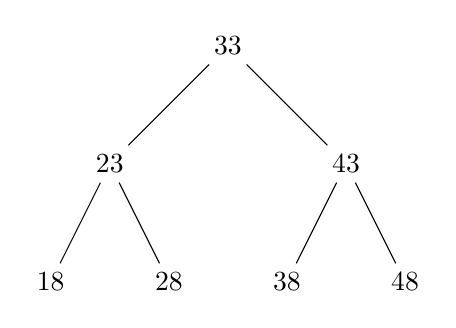
\begin{tikzpicture}[level distance=1.5cm,
  level 1/.style={sibling distance=3cm},
  level 2/.style={sibling distance=1.5cm}]
  \node {33}
    child {node {23}
      child {node {18}}
      child {node {28}}
    }
    child {node {43}
      child {node {38}}
      child {node {48}}
    };
\end{tikzpicture}
\caption{Пример бинарного дерева поиска}
\end{figure}

\item Написать программу на Python, которая реализует бинарное дерево поиска с инкапсуляцией. Программа должна создавать экземпляры класса KeyedNode, которые представляют узлы дерева, и класса ValuedTree, который представляет дерево поиска. Класс ValuedTree должен содержать методы для вставки, поиска и удаления элементов, при этом все рекурсивные методы должны быть приватными. Программа также должна создавать дерево поиска, вставлять в него случайные числа и выполнять поиск элементов в дереве.

Инструкции:
\begin{enumerate}
    \item Создайте класс KeyedNode с методом \_\_init\_\_, который принимает параметр keyed\_val и сохраняет его в атрибуте self.node\_content. Атрибуты self.left\_path и self.right\_path должны быть инициализированы как None.
    \item Создайте класс ValuedTree с методом \_\_init\_\_, который инициализирует атрибут self.root\_content как None.
    \item Создайте публичный метод insert\_content в классе ValuedTree, который вставляет значение в дерево. Если self.root\_content отсутствует, создайте новый узел с вставляемым значением. В противном случае, вызовите приватный метод \_insert\_content\_helper, передав ему self.root\_content и значение.
    \item Создайте приватный метод \_insert\_content\_helper в классе ValuedTree, который рекурсивно вставляет значение в дерево. Если значение меньше или равно значению текущего узла, вставьте его в левое поддерево. Если значение строго больше значения текущего узла, вставьте его в правое поддерево.
    \item Создайте публичный метод search\_content в классе ValuedTree, который ищет значение в дереве. Если дерево пустое, верните None. В противном случае, вызовите приватный метод \_search\_content\_helper, передав ему self.root\_content и искомое значение.
    \item Создайте приватный метод \_search\_content\_helper в классе ValuedTree, который рекурсивно ищет значение в дереве. Если текущий узел равен None или значение текущего узла равно искомому значению, верните текущий узел. В противном случае, рекурсивно вызывайте метод \_search\_content\_helper для поиска значения в левом поддереве (если искомое значение меньше или равно текущему) или в правом поддереве (если искомое значение больше).
    \item Создайте экземпляр класса ValuedTree и вставьте в него 31 случайное число от 11 до 51.
    \item Выполните поиск элементов в дереве и выведите результаты на экран.
\end{enumerate}

Пример использования:
\begin{lstlisting}[language=Python]
vt = ValuedTree()
for i in range(31):
    vt.insert_content(random.randint(11, 51))

print("Поиск элементов:")
print(vt.search_content(24))  # Обнаружено, возвращен узел (24)
print(vt.search_content(64))  # Не обнаружено, возвращено None
print(vt.search_content(44))  # Обнаружено, возвращен узел (44)
\end{lstlisting}

\begin{figure}[h]
\centering
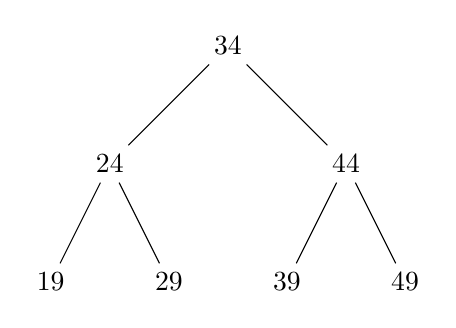
\begin{tikzpicture}[level distance=1.5cm,
  level 1/.style={sibling distance=3cm},
  level 2/.style={sibling distance=1.5cm}]
  \node {34}
    child {node {24}
      child {node {19}}
      child {node {29}}
    }
    child {node {44}
      child {node {39}}
      child {node {49}}
    };
\end{tikzpicture}
\caption{Пример бинарного дерева поиска}
\end{figure}

\item Написать программу на Python, которая реализует бинарное дерево поиска с инкапсуляцией. Программа должна создавать экземпляры класса ContentNode, которые представляют узлы дерева, и класса KeyTreeStructure, который представляет дерево поиска. Класс KeyTreeStructure должен содержать методы для вставки, поиска и удаления элементов, при этом все вспомогательные методы должны быть приватными. Программа также должна создавать дерево поиска, вставлять в него случайные числа и выполнять поиск элементов в дереве.

Инструкции:
\begin{enumerate}
    \item Создайте класс ContentNode с методом \_\_init\_\_, который принимает параметр content\_val и сохраняет его в атрибуте self.node\_data. Атрибуты self.left\_item и self.right\_item должны быть инициализированы как None.
    \item Создайте класс KeyTreeStructure с методом \_\_init\_\_, который инициализирует атрибут self.top\_data как None.
    \item Создайте публичный метод add\_data в классе KeyTreeStructure, который вставляет значение в дерево. Если self.top\_data отсутствует, создайте новый узел с вставляемым значением. В противном случае, вызовите приватный метод \_add\_data\_rec, передав ему self.top\_data и значение.
    \item Создайте приватный метод \_add\_data\_rec в классе KeyTreeStructure, который рекурсивно вставляет значение в дерево. Если значение строго меньше значения текущего узла, вставьте его в левое поддерево. Если значение больше или равно значению текущего узла, вставьте его в правое поддерево.
    \item Создайте публичный метод find\_data в классе KeyTreeStructure, который ищет значение в дереве. Если дерево пустое, верните None. В противном случае, вызовите приватный метод \_find\_data\_rec, передав ему self.top\_data и искомое значение.
    \item Создайте приватный метод \_find\_data\_rec в классе KeyTreeStructure, который рекурсивно ищет значение в дереве. Если текущий узел равен None или значение текущего узла равно искомому значению, верните текущий узел. В противном случае, рекурсивно вызывайте метод \_find\_data\_rec для поиска значения в левом поддереве (если искомое значение меньше текущего) или в правом поддереве (если искомое значение больше или равно текущему).
    \item Создайте экземпляр класса KeyTreeStructure и вставьте в него 32 случайных числа от 12 до 52.
    \item Выполните поиск элементов в дереве и выведите результаты на экран.
\end{enumerate}

Пример использования:
\begin{lstlisting}[language=Python]
kts = KeyTreeStructure()
for i in range(32):
    kts.add_data(random.randint(12, 52))

print("Поиск элементов:")
print(kts.find_data(25))  # Обнаружено, возвращен узел (25)
print(kts.find_data(65))  # Не обнаружено, возвращено None
print(kts.find_data(45))  # Обнаружено, возвращен узел (45)
\end{lstlisting}

\begin{figure}[h]
\centering
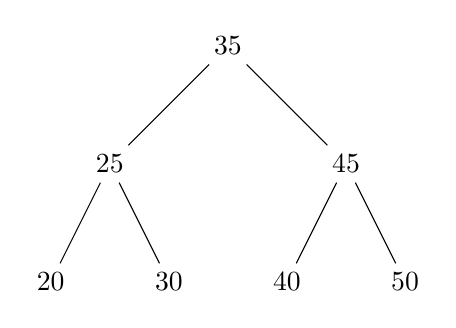
\begin{tikzpicture}[level distance=1.5cm,
  level 1/.style={sibling distance=3cm},
  level 2/.style={sibling distance=1.5cm}]
  \node {35}
    child {node {25}
      child {node {20}}
      child {node {30}}
    }
    child {node {45}
      child {node {40}}
      child {node {50}}
    };
\end{tikzpicture}
\caption{Пример бинарного дерева поиска}
\end{figure}

\item Написать программу на Python, которая реализует бинарное дерево поиска с инкапсуляцией. Программа должна создавать экземпляры класса DataNode, которые представляют узлы дерева, и класса ContentTree, который представляет дерево поиска. Класс ContentTree должен содержать методы для вставки, поиска и удаления элементов, при этом все рекурсивные методы должны быть приватными. Программа также должна создавать дерево поиска, вставлять в него случайные числа и выполнять поиск элементов в дереве.

Инструкции:
\begin{enumerate}
    \item Создайте класс DataNode с методом \_\_init\_\_, который принимает параметр data\_value и сохраняет его в атрибуте self.tree\_content. Атрибуты self.left\_entry и self.right\_entry должны быть инициализированы как None.
    \item Создайте класс ContentTree с методом \_\_init\_\_, который инициализирует атрибут self.root\_content как None.
    \item Создайте публичный метод insert\_entry в классе ContentTree, который вставляет значение в дерево. Если self.root\_content отсутствует, создайте новый узел с вставляемым значением. В противном случае, вызовите приватный метод \_insert\_entry\_helper, передав ему self.root\_content и значение.
    \item Создайте приватный метод \_insert\_entry\_helper в классе ContentTree, который рекурсивно вставляет значение в дерево. Если значение меньше или равно значению текущего узла, вставьте его в левое поддерево. Если значение строго больше значения текущего узла, вставьте его в правое поддерево.
    \item Создайте публичный метод search\_entry в классе ContentTree, который ищет значение в дереве. Если дерево пустое, верните None. В противном случае, вызовите приватный метод \_search\_entry\_helper, передав ему self.root\_content и искомое значение.
    \item Создайте приватный метод \_search\_entry\_helper в классе ContentTree, который рекурсивно ищет значение в дереве. Если текущий узел равен None или значение текущего узла равно искомому значению, верните текущий узел. В противном случае, рекурсивно вызывайте метод \_search\_entry\_helper для поиска значения в левом поддереве (если искомое значение меньше или равно текущему) или в правом поддереве (если искомое значение больше).
    \item Создайте экземпляр класса ContentTree и вставьте в него 33 случайных числа от 13 до 53.
    \item Выполните поиск элементов в дереве и выведите результаты на экран.
\end{enumerate}

Пример использования:
\begin{lstlisting}[language=Python]
ct = ContentTree()
for i in range(33):
    ct.insert_entry(random.randint(13, 53))

print("Поиск элементов:")
print(ct.search_entry(26))  # Обнаружено, возвращен узел (26)
print(ct.search_entry(66))  # Не обнаружено, возвращено None
print(ct.search_entry(46))  # Обнаружено, возвращен узел (46)
\end{lstlisting}

\begin{figure}[h]
\centering
\begin{tikzpicture}[level distance=1.5cm,
  level 1/.style={sibling distance=3cm},
  level 2/.style={sibling distance=1.5cm}]
  \node {36}
    child {node {26}
      child {node {21}}
      child {node {31}}
    }
    child {node {46}
      child {node {41}}
      child {node {51}}
    };
\end{tikzpicture}
\caption{Пример бинарного дерева поиска}
\end{figure}

\item Написать программу на Python, которая реализует бинарное дерево поиска с инкапсуляцией. Программа должна создавать экземпляры класса EntryNode, которые представляют узлы дерева, и класса DataStructureTree, который представляет дерево поиска. Класс DataStructureTree должен содержать методы для вставки, поиска и удаления элементов, при этом все вспомогательные методы должны быть приватными. Программа также должна создавать дерево поиска, вставлять в него случайные числа и выполнять поиск элементов в дереве.

Инструкции:
\begin{enumerate}
    \item Создайте класс EntryNode с методом \_\_init\_\_, который принимает параметр entry\_val и сохраняет его в атрибуте self.content\_item. Атрибуты self.left\_data и self.right\_data должны быть инициализированы как None.
    \item Создайте класс DataStructureTree с методом \_\_init\_\_, который инициализирует атрибут self.first\_item как None.
    \item Создайте публичный метод add\_item в классе DataStructureTree, который вставляет значение в дерево. Если self.first\_item отсутствует, создайте новый узел с вставляемым значением. В противном случае, вызовите приватный метод \_add\_item\_rec, передав ему self.first\_item и значение.
    \item Создайте приватный метод \_add\_item\_rec в классе DataStructureTree, который рекурсивно вставляет значение в дерево. Если значение строго меньше значения текущего узла, вставьте его в левое поддерево. Если значение больше или равно значению текущего узла, вставьте его в правое поддерево.
    \item Создайте публичный метод locate\_item в классе DataStructureTree, который ищет значение в дереве. Если дерево пустое, верните None. В противном случае, вызовите приватный метод \_locate\_item\_rec, передав ему self.first\_item и искомое значение.
    \item Создайте приватный метод \_locate\_item\_rec в классе DataStructureTree, который рекурсивно ищет значение в дереве. Если текущий узел равен None или значение текущего узла равно искомому значению, верните текущий узел. В противном случае, рекурсивно вызывайте метод \_locate\_item\_rec для поиска значения в левом поддереве (если искомое значение меньше текущего) или в правом поддереве (если искомое значение больше или равно текущему).
    \item Создайте экземпляр класса DataStructureTree и вставьте в него 34 случайных числа от 14 до 54.
    \item Выполните поиск элементов в дереве и выведите результаты на экран.
\end{enumerate}

Пример использования:
\begin{lstlisting}[language=Python]
dst = DataStructureTree()
for i in range(34):
    dst.add_item(random.randint(14, 54))

print("Поиск элементов:")
print(dst.locate_item(27))  # Обнаружено, возвращен узел (27)
print(dst.locate_item(67))  # Не обнаружено, возвращено None
print(dst.locate_item(47))  # Обнаружено, возвращен узел (47)
\end{lstlisting}

\begin{figure}[h]
\centering
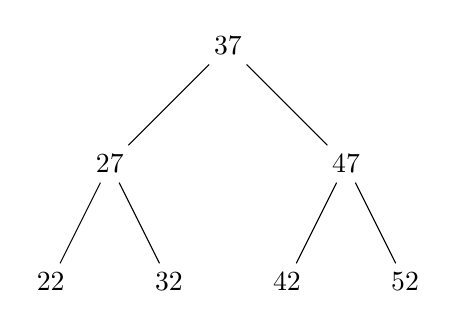
\begin{tikzpicture}[level distance=1.5cm,
  level 1/.style={sibling distance=3cm},
  level 2/.style={sibling distance=1.5cm}]
  \node {37}
    child {node {27}
      child {node {22}}
      child {node {32}}
    }
    child {node {47}
      child {node {42}}
      child {node {52}}
    };
\end{tikzpicture}
\caption{Пример бинарного дерева поиска}
\end{figure}

\item Написать программу на Python, которая реализует бинарное дерево поиска с инкапсуляцией. Программа должна создавать экземпляры класса ItemNode, которые представляют узлы дерева, и класса EntryTree, который представляет дерево поиска. Класс EntryTree должен содержать методы для вставки, поиска и удаления элементов, при этом все рекурсивные методы должны быть приватными. Программа также должна создавать дерево поиска, вставлять в него случайные числа и выполнять поиск элементов в дереве.

Инструкции:
\begin{enumerate}
    \item Создайте класс ItemNode с методом \_\_init\_\_, который принимает параметр item\_value и сохраняет его в атрибуте self.data\_entry. Атрибуты self.left\_position и self.right\_position должны быть инициализированы как None.
    \item Создайте класс EntryTree с методом \_\_init\_\_, который инициализирует атрибут self.root\_entry как None.
    \item Создайте публичный метод insert\_position в классе EntryTree, который вставляет значение в дерево. Если self.root\_entry отсутствует, создайте новый узел с вставляемым значением. В противном случае, вызовите приватный метод \_insert\_position\_helper, передав ему self.root\_entry и значение.
    \item Создайте приватный метод \_insert\_position\_helper в классе EntryTree, который рекурсивно вставляет значение в дерево. Если значение меньше или равно значению текущего узла, вставьте его в левое поддерево. Если значение строго больше значения текущего узла, вставьте его в правое поддерево.
    \item Создайте публичный метод find\_position в классе EntryTree, который ищет значение в дереве. Если дерево пустое, верните None. В противном случае, вызовите приватный метод \_find\_position\_helper, передав ему self.root\_entry и искомое значение.
    \item Создайте приватный метод \_find\_position\_helper в классе EntryTree, который рекурсивно ищет значение в дереве. Если текущий узел равен None или значение текущего узла равно искомому значению, верните текущий узел. В противном случае, рекурсивно вызывайте метод \_find\_position\_helper для поиска значения в левом поддереве (если искомое значение меньше или равно текущему) или в правом поддереве (если искомое значение больше).
    \item Создайте экземпляр класса EntryTree и вставьте в него 35 случайных чисел от 15 до 55.
    \item Выполните поиск элементов в дереве и выведите результаты на экран.
\end{enumerate}

Пример использования:
\begin{lstlisting}[language=Python]
et = EntryTree()
for i in range(35):
    et.insert_position(random.randint(15, 55))

print("Поиск элементов:")
print(et.find_position(28))  # Обнаружено, возвращен узел (28)
print(et.find_position(68))  # Не обнаружено, возвращено None
print(et.find_position(48))  # Обнаружено, возвращен узел (48)
\end{lstlisting}

\begin{figure}[h]
\centering
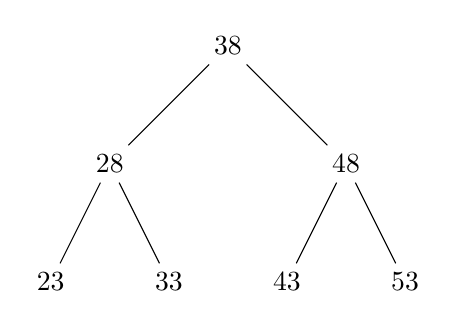
\begin{tikzpicture}[level distance=1.5cm,
  level 1/.style={sibling distance=3cm},
  level 2/.style={sibling distance=1.5cm}]
  \node {38}
    child {node {28}
      child {node {23}}
      child {node {33}}
    }
    child {node {48}
      child {node {43}}
      child {node {53}}
    };
\end{tikzpicture}
\caption{Пример бинарного дерева поиска}
\end{figure}

\item Написать программу на Python, которая реализует бинарное дерево поиска с инкапсуляцией. Программа должна создавать экземпляры класса PositionNode, которые представляют узлы дерева, и класса ItemStructure, который представляет дерево поиска. Класс ItemStructure должен содержать методы для вставки, поиска и удаления элементов, при этом все вспомогательные методы должны быть приватными. Программа также должна создавать дерево поиска, вставлять в него случайные числа и выполнять поиск элементов в дереве.

Инструкции:
\begin{enumerate}
    \item Создайте класс PositionNode с методом \_\_init\_\_, который принимает параметр position\_val и сохраняет его в атрибуте self.entry\_data. Атрибуты self.left\_slot и self.right\_slot должны быть инициализированы как None.
    \item Создайте класс ItemStructure с методом \_\_init\_\_, который инициализирует атрибут self.top\_entry как None.
    \item Создайте публичный метод add\_slot в классе ItemStructure, который вставляет значение в дерево. Если self.top\_entry отсутствует, создайте новый узел с вставляемым значением. В противном случае, вызовите приватный метод \_add\_slot\_rec, передав ему self.top\_entry и значение.
    \item Создайте приватный метод \_add\_slot\_rec в классе ItemStructure, который рекурсивно вставляет значение в дерево. Если значение строго меньше значения текущего узла, вставьте его в левое поддерево. Если значение больше или равно значению текущего узла, вставьте его в правое поддерево.
    \item Создайте публичный метод search\_slot в классе ItemStructure, который ищет значение в дереве. Если дерево пустое, верните None. В противном случае, вызовите приватный метод \_search\_slot\_rec, передав ему self.top\_entry и искомое значение.
    \item Создайте приватный метод \_search\_slot\_rec в классе ItemStructure, который рекурсивно ищет значение в дереве. Если текущий узел равен None или значение текущего узла равно искомому значению, верните текущий узел. В противном случае, рекурсивно вызывайте метод \_search\_slot\_rec для поиска значения в левом поддереве (если искомое значение меньше текущего) или в правом поддереве (если искомое значение больше или равно текущему).
    \item Создайте экземпляр класса ItemStructure и вставьте в него 36 случайных чисел от 16 до 56.
    \item Выполните поиск элементов в дереве и выведите результаты на экран.
\end{enumerate}

Пример использования:
\begin{lstlisting}[language=Python]
is_ = ItemStructure()
for i in range(36):
    is_.add_slot(random.randint(16, 56))

print("Поиск элементов:")
print(is_.search_slot(29))  # Обнаружено, возвращен узел (29)
print(is_.search_slot(69))  # Не обнаружено, возвращено None
print(is_.search_slot(49))  # Обнаружено, возвращен узел (49)
\end{lstlisting}

\begin{figure}[h]
\centering
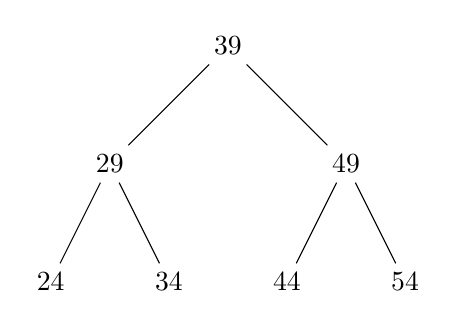
\begin{tikzpicture}[level distance=1.5cm,
  level 1/.style={sibling distance=3cm},
  level 2/.style={sibling distance=1.5cm}]
  \node {39}
    child {node {29}
      child {node {24}}
      child {node {34}}
    }
    child {node {49}
      child {node {44}}
      child {node {54}}
    };
\end{tikzpicture}
\caption{Пример бинарного дерева поиска}
\end{figure}

\item Написать программу на Python, которая реализует бинарное дерево поиска с инкапсуляцией. Программа должна создавать экземпляры класса SlotNode, которые представляют узлы дерева, и класса PositionTree, который представляет дерево поиска. Класс PositionTree должен содержать методы для вставки, поиска и удаления элементов, при этом все рекурсивные методы должны быть приватными. Программа также должна создавать дерево поиска, вставлять в него случайные числа и выполнять поиск элементов в дереве.

Инструкции:
\begin{enumerate}
    \item Создайте класс SlotNode с методом \_\_init\_\_, который принимает параметр slot\_value и сохраняет его в атрибуте self.item\_position. Атрибуты self.left\_place и self.right\_place должны быть инициализированы как None.
    \item Создайте класс PositionTree с методом \_\_init\_\_, который инициализирует атрибут self.first\_position как None.
    \item Создайте публичный метод insert\_place в классе PositionTree, который вставляет значение в дерево. Если self.first\_position отсутствует, создайте новый узел с вставляемым значением. В противном случае, вызовите приватный метод \_insert\_place\_helper, передав ему self.first\_position и значение.
    \item Создайте приватный метод \_insert\_place\_helper в классе PositionTree, который рекурсивно вставляет значение в дерево. Если значение меньше или равно значению текущего узла, вставьте его в левое поддерево. Если значение строго больше значения текущего узла, вставьте его в правое поддерево.
    \item Создайте публичный метод locate\_place в классе PositionTree, который ищет значение в дереве. Если дерево пустое, верните None. В противном случае, вызовите приватный метод \_locate\_place\_helper, передав ему self.first\_position и искомое значение.
    \item Создайте приватный метод \_locate\_place\_helper в классе PositionTree, который рекурсивно ищет значение в дереве. Если текущий узел равен None или значение текущего узла равно искомому значению, верните текущий узел. В противном случае, рекурсивно вызывайте метод \_locate\_place\_helper для поиска значения в левом поддереве (если искомое значение меньше или равно текущему) или в правом поддереве (если искомое значение больше).
    \item Создайте экземпляр класса PositionTree и вставьте в него 37 случайных чисел от 17 до 57.
    \item Выполните поиск элементов в дереве и выведите результаты на экран.
\end{enumerate}

Пример использования:
\begin{lstlisting}[language=Python]
pt = PositionTree()
for i in range(37):
    pt.insert_place(random.randint(17, 57))

print("Поиск элементов:")
print(pt.locate_place(30))  # Обнаружено, возвращен узел (30)
print(pt.locate_place(70))  # Не обнаружено, возвращено None
print(pt.locate_place(50))  # Обнаружено, возвращен узел (50)
\end{lstlisting}

\begin{figure}[h]
\centering
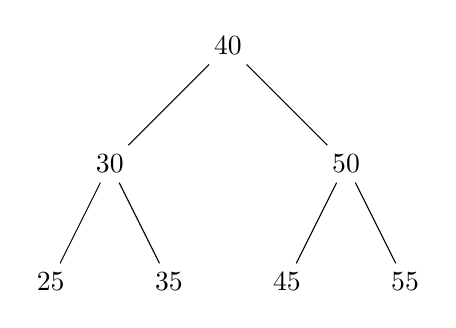
\begin{tikzpicture}[level distance=1.5cm,
  level 1/.style={sibling distance=3cm},
  level 2/.style={sibling distance=1.5cm}]
  \node {40}
    child {node {30}
      child {node {25}}
      child {node {35}}
    }
    child {node {50}
      child {node {45}}
      child {node {55}}
    };
\end{tikzpicture}
\caption{Пример бинарного дерева поиска}
\end{figure}

\item Написать программу на Python, которая реализует бинарное дерево поиска с инкапсуляцией. Программа должна создавать экземпляры класса PlaceNode, которые представляют узлы дерева, и класса SlotTree, который представляет дерево поиска. Класс SlotTree должен содержать методы для вставки, поиска и удаления элементов, при этом все вспомогательные методы должны быть приватными. Программа также должна создавать дерево поиска, вставлять в него случайные числа и выполнять поиск элементов в дереве.

Инструкции:
\begin{enumerate}
    \item Создайте класс PlaceNode с методом \_\_init\_\_, который принимает параметр place\_val и сохраняет его в атрибуте self.position\_item. Атрибуты self.left\_spot и self.right\_spot должны быть инициализированы как None.
    \item Создайте класс SlotTree с методом \_\_init\_\_, который инициализирует атрибут self.root\_position как None.
    \item Создайте публичный метод add\_spot в классе SlotTree, который вставляет значение в дерево. Если self.root\_position отсутствует, создайте новый узел с вставляемым значением. В противном случае, вызовите приватный метод \_add\_spot\_rec, передав ему self.root\_position и значение.
    \item Создайте приватный метод \_add\_spot\_rec в классе SlotTree, который рекурсивно вставляет значение в дерево. Если значение строго меньше значения текущего узла, вставьте его в левое поддерево. Если значение больше или равно значению текущего узла, вставьте его в правое поддерево.
    \item Создайте публичный метод find\_spot в классе SlotTree, который ищет значение в дереве. Если дерево пустое, верните None. В противном случае, вызовите приватный метод \_find\_spot\_rec, передав ему self.root\_position и искомое значение.
    \item Создайте приватный метод \_find\_spot\_rec в классе SlotTree, который рекурсивно ищет значение в дереве. Если текущий узел равен None или значение текущего узла равно искомому значению, верните текущий узел. В противном случае, рекурсивно вызывайте метод \_find\_spot\_rec для поиска значения в левом поддереве (если искомое значение меньше текущего) или в правом поддереве (если искомое значение больше или равно текущему).
    \item Создайте экземпляр класса SlotTree и вставьте в него 38 случайных чисел от 18 до 58.
    \item Выполните поиск элементов в дереве и выведите результаты на экран.
\end{enumerate}

Пример использования:
\begin{lstlisting}[language=Python]
st = SlotTree()
for i in range(38):
    st.add_spot(random.randint(18, 58))

print("Поиск элементов:")
print(st.find_spot(31))  # Обнаружено, возвращен узел (31)
print(st.find_spot(71))  # Не обнаружено, возвращено None
print(st.find_spot(51))  # Обнаружено, возвращен узел (51)
\end{lstlisting}

\begin{figure}[h]
\centering
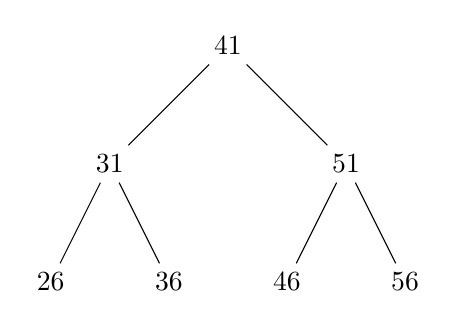
\begin{tikzpicture}[level distance=1.5cm,
  level 1/.style={sibling distance=3cm},
  level 2/.style={sibling distance=1.5cm}]
  \node {41}
    child {node {31}
      child {node {26}}
      child {node {36}}
    }
    child {node {51}
      child {node {46}}
      child {node {56}}
    };
\end{tikzpicture}
\caption{Пример бинарного дерева поиска}
\end{figure}

\item Написать программу на Python, которая реализует бинарное дерево поиска с инкапсуляцией. Программа должна создавать экземпляры класса SpotNode, которые представляют узлы дерева, и класса PlaceIndex, который представляет дерево поиска. Класс PlaceIndex должен содержать методы для вставки, поиска и удаления элементов, при этом все рекурсивные методы должны быть приватными. Программа также должна создавать дерево поиска, вставлять в него случайные числа и выполнять поиск элементов в дереве.

Инструкции:
\begin{enumerate}
    \item Создайте класс SpotNode с методом \_\_init\_\_, который принимает параметр spot\_value и сохраняет его в атрибуте self.index\_position. Атрибуты self.left\_location и self.right\_location должны быть инициализированы как None.
    \item Создайте класс PlaceIndex с методом \_\_init\_\_, который инициализирует атрибут self.start\_position как None.
    \item Создайте публичный метод insert\_location в классе PlaceIndex, который вставляет значение в дерево. Если self.start\_position отсутствует, создайте новый узел с вставляемым значением. В противном случае, вызовите приватный метод \_insert\_location\_helper, передав ему self.start\_position и значение.
    \item Создайте приватный метод \_insert\_location\_helper в классе PlaceIndex, который рекурсивно вставляет значение в дерево. Если значение меньше или равно значению текущего узла, вставьте его в левое поддерево. Если значение строго больше значения текущего узла, вставьте его в правое поддерево.
    \item Создайте публичный метод search\_location в классе PlaceIndex, который ищет значение в дереве. Если дерево пустое, верните None. В противном случае, вызовите приватный метод \_search\_location\_helper, передав ему self.start\_position и искомое значение.
    \item Создайте приватный метод \_search\_location\_helper в классе PlaceIndex, который рекурсивно ищет значение в дереве. Если текущий узел равен None или значение текущего узла равно искомому значению, верните текущий узел. В противном случае, рекурсивно вызывайте метод \_search\_location\_helper для поиска значения в левом поддереве (если искомое значение меньше или равно текущему) или в правом поддереве (если искомое значение больше).
    \item Создайте экземпляр класса PlaceIndex и вставьте в него 39 случайных чисел от 19 до 59.
    \item Выполните поиск элементов в дереве и выведите результаты на экран.
\end{enumerate}

Пример использования:
\begin{lstlisting}[language=Python]
pi = PlaceIndex()
for i in range(39):
    pi.insert_location(random.randint(19, 59))

print("Поиск элементов:")
print(pi.search_location(32))  # Обнаружено, возвращен узел (32)
print(pi.search_location(72))  # Не обнаружено, возвращено None
print(pi.search_location(52))  # Обнаружено, возвращен узел (52)
\end{lstlisting}

\begin{figure}[h]
\centering
\begin{tikzpicture}[level distance=1.5cm,
  level 1/.style={sibling distance=3cm},
  level 2/.style={sibling distance=1.5cm}]
  \node {42}
    child {node {32}
      child {node {27}}
      child {node {37}}
    }
    child {node {52}
      child {node {47}}
      child {node {57}}
    };
\end{tikzpicture}
\caption{Пример бинарного дерева поиска}
\end{figure}

\item Написать программу на Python, которая реализует бинарное дерево поиска с инкапсуляцией. Программа должна создавать экземпляры класса LocationNode, которые представляют узлы дерева, и класса SpotTree, который представляет дерево поиска. Класс SpotTree должен содержать методы для вставки, поиска и удаления элементов, при этом все вспомогательные методы должны быть приватными. Программа также должна создавать дерево поиска, вставлять в него случайные числа и выполнять поиск элементов в дереве.

Инструкции:
\begin{enumerate}
    \item Создайте класс LocationNode с методом \_\_init\_\_, который принимает параметр location\_val и сохраняет его в атрибуте self.tree\_spot. Атрибуты self.left\_site и self.right\_site должны быть инициализированы как None.
    \item Создайте класс SpotTree с методом \_\_init\_\_, который инициализирует атрибут self.base\_spot как None.
    \item Создайте публичный метод add\_site в классе SpotTree, который вставляет значение в дерево. Если self.base\_spot отсутствует, создайте новый узел с вставляемым значением. В противном случае, вызовите приватный метод \_add\_site\_rec, передав ему self.base\_spot и значение.
    \item Создайте приватный метод \_add\_site\_rec в классе SpotTree, который рекурсивно вставляет значение в дерево. Если значение строго меньше значения текущего узла, вставьте его в левое поддерево. Если значение больше или равно значению текущего узла, вставьте его в правое поддерево.
    \item Создайте публичный метод locate\_site в классе SpotTree, который ищет значение в дереве. Если дерево пустое, верните None. В противном случае, вызовите приватный метод \_locate\_site\_rec, передав ему self.base\_spot и искомое значение.
    \item Создайте приватный метод \_locate\_site\_rec в классе SpotTree, который рекурсивно ищет значение в дереве. Если текущий узел равен None или значение текущего узла равно искомому значению, верните текущий узел. В противном случае, рекурсивно вызывайте метод \_locate\_site\_rec для поиска значения в левом поддереве (если искомое значение меньше текущего) или в правом поддереве (если искомое значение больше или равно текущему).
    \item Создайте экземпляр класса SpotTree и вставьте в него 40 случайных чисел от 20 до 60.
    \item Выполните поиск элементов в дереве и выведите результаты на экран.
\end{enumerate}

Пример использования:
\begin{lstlisting}[language=Python]
spot_tree = SpotTree()
for i in range(40):
    spot_tree.add_site(random.randint(20, 60))

print("Поиск элементов:")
print(spot_tree.locate_site(33))  # Обнаружено, возвращен узел (33)
print(spot_tree.locate_site(73))  # Не обнаружено, возвращено None
print(spot_tree.locate_site(53))  # Обнаружено, возвращен узел (53)
\end{lstlisting}

\begin{figure}[h]
\centering
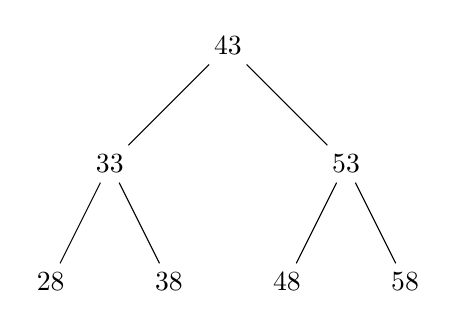
\begin{tikzpicture}[level distance=1.5cm,
  level 1/.style={sibling distance=3cm},
  level 2/.style={sibling distance=1.5cm}]
  \node {43}
    child {node {33}
      child {node {28}}
      child {node {38}}
    }
    child {node {53}
      child {node {48}}
      child {node {58}}
    };
\end{tikzpicture}
\caption{Пример бинарного дерева поиска}
\end{figure}

\item Написать программу на Python, которая реализует бинарное дерево поиска с инкапсуляцией. Программа должна создавать экземпляры класса SiteNode, которые представляют узлы дерева, и класса LocationIndex, который представляет дерево поиска. Класс LocationIndex должен содержать методы для вставки, поиска и удаления элементов, при этом все рекурсивные методы должны быть приватными. Программа также должна создавать дерево поиска, вставлять в него случайные числа и выполнять поиск элементов в дереве.

Инструкции:
\begin{enumerate}
    \item Создайте класс SiteNode с методом \_\_init\_\_, который принимает параметр site\_value и сохраняет его в атрибуте self.index\_location. Атрибуты self.left\_zone и self.right\_zone должны быть инициализированы как None.
    \item Создайте класс LocationIndex с методом \_\_init\_\_, который инициализирует атрибут self.root\_location как None.
    \item Создайте публичный метод insert\_zone в классе LocationIndex, который вставляет значение в дерево. Если self.root\_location отсутствует, создайте новый узел с вставляемым значением. В противном случае, вызовите приватный метод \_insert\_zone\_helper, передав ему self.root\_location и значение.
    \item Создайте приватный метод \_insert\_zone\_helper в классе LocationIndex, который рекурсивно вставляет значение в дерево. Если значение меньше или равно значению текущего узла, вставьте его в левое поддерево. Если значение строго больше значения текущего узла, вставьте его в правое поддерево.
    \item Создайте публичный метод find\_zone в классе LocationIndex, который ищет значение в дереве. Если дерево пустое, верните None. В противном случае, вызовите приватный метод \_find\_zone\_helper, передав ему self.root\_location и искомое значение.
    \item Создайте приватный метод \_find\_zone\_helper в классе LocationIndex, который рекурсивно ищет значение в дереве. Если текущий узел равен None или значение текущего узла равно искомому значению, верните текущий узел. В противном случае, рекурсивно вызывайте метод \_find\_zone\_helper для поиска значения в левом поддереве (если искомое значение меньше или равно текущему) или в правом поддереве (если искомое значение больше).
    \item Создайте экземпляр класса LocationIndex и вставьте в него 41 случайное число от 21 до 61.
    \item Выполните поиск элементов в дереве и выведите результаты на экран.
\end{enumerate}

Пример использования:
\begin{lstlisting}[language=Python]
li = LocationIndex()
for i in range(41):
    li.insert_zone(random.randint(21, 61))

print("Поиск элементов:")
print(li.find_zone(34))  # Обнаружено, возвращен узел (34)
print(li.find_zone(74))  # Не обнаружено, возвращено None
print(li.find_zone(54))  # Обнаружено, возвращен узел (54)
\end{lstlisting}

\begin{figure}[h]
\centering
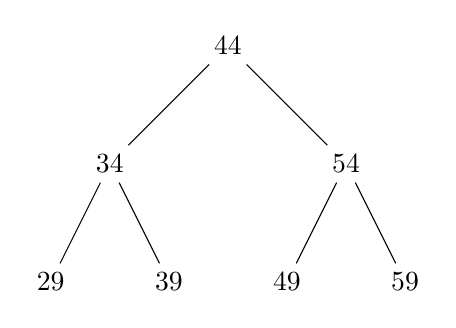
\begin{tikzpicture}[level distance=1.5cm,
  level 1/.style={sibling distance=3cm},
  level 2/.style={sibling distance=1.5cm}]
  \node {44}
    child {node {34}
      child {node {29}}
      child {node {39}}
    }
    child {node {54}
      child {node {49}}
      child {node {59}}
    };
\end{tikzpicture}
\caption{Пример бинарного дерева поиска}
\end{figure}

\item Написать программу на Python, которая реализует бинарное дерево поиска с инкапсуляцией. Программа должна создавать экземпляры класса ZoneNode, которые представляют узлы дерева, и класса SiteStructure, который представляет дерево поиска. Класс SiteStructure должен содержать методы для вставки, поиска и удаления элементов, при этом все вспомогательные методы должны быть приватными. Программа также должна создавать дерево поиска, вставлять в него случайные числа и выполнять поиск элементов в дереве.

Инструкции:
\begin{enumerate}
    \item Создайте класс ZoneNode с методом \_\_init\_\_, который принимает параметр zone\_val и сохраняет его в атрибуте self.structure\_site. Атрибуты self.left\_region и self.right\_region должны быть инициализированы как None.
    \item Создайте класс SiteStructure с методом \_\_init\_\_, который инициализирует атрибут self.top\_site как None.
    \item Создайте публичный метод add\_region в классе SiteStructure, который вставляет значение в дерево. Если self.top\_site отсутствует, создайте новый узел с вставляемым значением. В противном случае, вызовите приватный метод \_add\_region\_rec, передав ему self.top\_site и значение.
    \item Создайте приватный метод \_add\_region\_rec в классе SiteStructure, который рекурсивно вставляет значение в дерево. Если значение строго меньше значения текущего узла, вставьте его в левое поддерево. Если значение больше или равно значению текущего узла, вставьте его в правое поддерево.
    \item Создайте публичный метод search\_region в классе SiteStructure, который ищет значение в дереве. Если дерево пустое, верните None. В противном случае, вызовите приватный метод \_search\_region\_rec, передав ему self.top\_site и искомое значение.
    \item Создайте приватный метод \_search\_region\_rec в классе SiteStructure, который рекурсивно ищет значение в дереве. Если текущий узел равен None или значение текущего узла равно искомому значению, верните текущий узел. В противном случае, рекурсивно вызывайте метод \_search\_region\_rec для поиска значения в левом поддереве (если искомое значение меньше текущего) или в правом поддереве (если искомое значение больше или равно текущему).
    \item Создайте экземпляр класса SiteStructure и вставьте в него 42 случайных числа от 22 до 62.
    \item Выполните поиск элементов в дереве и выведите результаты на экран.
\end{enumerate}

Пример использования:
\begin{lstlisting}[language=Python]
ss = SiteStructure()
for i in range(42):
    ss.add_region(random.randint(22, 62))

print("Поиск элементов:")
print(ss.search_region(35))  # Обнаружено, возвращен узел (35)
print(ss.search_region(75))  # Не обнаружено, возвращено None
print(ss.search_region(55))  # Обнаружено, возвращен узел (55)
\end{lstlisting}

\begin{figure}[h]
\centering
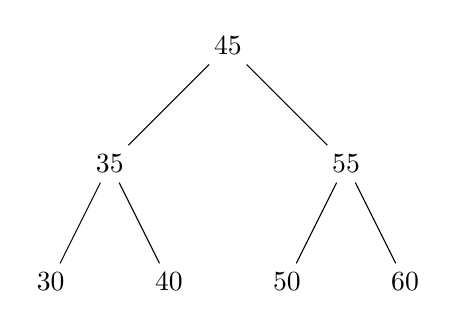
\begin{tikzpicture}[level distance=1.5cm,
  level 1/.style={sibling distance=3cm},
  level 2/.style={sibling distance=1.5cm}]
  \node {45}
    child {node {35}
      child {node {30}}
      child {node {40}}
    }
    child {node {55}
      child {node {50}}
      child {node {60}}
    };
\end{tikzpicture}
\caption{Пример бинарного дерева поиска}
\end{figure}

\item Написать программу на Python, которая реализует бинарное дерево поиска с инкапсуляцией. Программа должна создавать экземпляры класса RegionNode, которые представляют узлы дерева, и класса ZoneTree, который представляет дерево поиска. Класс ZoneTree должен содержать методы для вставки, поиска и удаления элементов, при этом все рекурсивные методы должны быть приватными. Программа также должна создавать дерево поиска, вставлять в него случайные числа и выполнять поиск элементов в дереве.

Инструкции:
\begin{enumerate}
    \item Создайте класс RegionNode с методом \_\_init\_\_, который принимает параметр region\_value и сохраняет его в атрибуте self.tree\_zone. Атрибуты self.left\_area и self.right\_area должны быть инициализированы как None.
    \item Создайте класс ZoneTree с методом \_\_init\_\_, который инициализирует атрибут self.first\_zone как None.
    \item Создайте публичный метод insert\_area в классе ZoneTree, который вставляет значение в дерево. Если self.first\_zone отсутствует, создайте новый узел с вставляемым значением. В противном случае, вызовите приватный метод \_insert\_area\_helper, передав ему self.first\_zone и значение.
    \item Создайте приватный метод \_insert\_area\_helper в классе ZoneTree, который рекурсивно вставляет значение в дерево. Если значение меньше или равно значению текущего узла, вставьте его в левое поддерево. Если значение строго больше значения текущего узла, вставьте его в правое поддерево.
    \item Создайте публичный метод locate\_area в классе ZoneTree, который ищет значение в дереве. Если дерево пустое, верните None. В противном случае, вызовите приватный метод \_locate\_area\_rec, передав ему self.first\_zone и искомое значение.
    \item Создайте приватный метод \_locate\_area\_rec в классе ZoneTree, который рекурсивно ищет значение в дереве. Если текущий узел равен None или значение текущего узла равно искомому значению, верните текущий узел. В противном случае, рекурсивно вызывайте метод \_locate\_area\_rec для поиска значения в левом поддереве (если искомое значение меньше или равно текущему) или в правом поддереве (если искомое значение больше).
    \item Создайте экземпляр класса ZoneTree и вставьте в него 43 случайных числа от 23 до 63.
    \item Выполните поиск элементов в дереве и выведите результаты на экран.
\end{enumerate}

Пример использования:
\begin{lstlisting}[language=Python]
zt = ZoneTree()
for i in range(43):
    zt.insert_area(random.randint(23, 63))

print("Поиск элементов:")
print(zt.locate_area(36))  # Обнаружено, возвращен узел (36)
print(zt.locate_area(76))  # Не обнаружено, возвращено None
print(zt.locate_area(56))  # Обнаружено, возвращен узел (56)
\end{lstlisting}

\begin{figure}[h]
\centering
\begin{tikzpicture}[level distance=1.5cm,
  level 1/.style={sibling distance=3cm},
  level 2/.style={sibling distance=1.5cm}]
  \node {46}
    child {node {36}
      child {node {31}}
      child {node {41}}
    }
    child {node {56}
      child {node {51}}
      child {node {61}}
    };
\end{tikzpicture}
\caption{Пример бинарного дерева поиска}
\end{figure}

\item Написать программу на Python, которая реализует бинарное дерево поиска с инкапсуляцией. Программа должна создавать экземпляры класса AreaNode, которые представляют узлы дерева, и класса RegionIndex, который представляет дерево поиска. Класс RegionIndex должен содержать методы для вставки, поиска и удаления элементов, при этом все вспомогательные методы должны быть приватными. Программа также должна создавать дерево поиска, вставлять в него случайные числа и выполнять поиск элементов в дереве.

Инструкции:
\begin{enumerate}
    \item Создайте класс AreaNode с методом \_\_init\_\_, который принимает параметр area\_val и сохраняет его в атрибуте self.index\_region. Атрибуты self.left\_district и self.right\_district должны быть инициализированы как None.
    \item Создайте класс RegionIndex с методом \_\_init\_\_, который инициализирует атрибут self.root\_region как None.
    \item Создайте публичный метод add\_district в классе RegionIndex, который вставляет значение в дерево. Если self.root\_region отсутствует, создайте новый узел с вставляемым значением. В противном случае, вызовите приватный метод \_add\_district\_rec, передав ему self.root\_region и значение.
    \item Создайте приватный метод \_add\_district\_rec в классе RegionIndex, который рекурсивно вставляет значение в дерево. Если значение строго меньше значения текущего узла, вставьте его в левое поддерево. Если значение больше или равно значению текущего узла, вставьте его в правое поддерево.
    \item Создайте публичный метод find\_district в классе RegionIndex, который ищет значение в дереве. Если дерево пустое, верните None. В противном случае, вызовите приватный метод \_find\_district\_helper, передав ему self.root\_region и искомое значение.
    \item Создайте приватный метод \_find\_district\_helper в классе RegionIndex, который рекурсивно ищет значение в дереве. Если текущий узел равен None или значение текущего узла равно искомому значению, верните текущий узел. В противном случае, рекурсивно вызывайте метод \_find\_district\_helper для поиска значения в левом поддереве (если искомое значение меньше текущего) или в правом поддереве (если искомое значение больше или равно текущему).
    \item Создайте экземпляр класса RegionIndex и вставьте в него 44 случайных числа от 24 до 64.
    \item Выполните поиск элементов в дереве и выведите результаты на экран.
\end{enumerate}

Пример использования:
\begin{lstlisting}[language=Python]
ri = RegionIndex()
for i in range(44):
    ri.add_district(random.randint(24, 64))

print("Поиск элементов:")
print(ri.find_district(37))  # Обнаружено, возвращен узел (37)
print(ri.find_district(77))  # Не обнаружено, возвращено None
print(ri.find_district(57))  # Обнаружено, возвращен узел (57)
\end{lstlisting}

\begin{figure}[h]
\centering
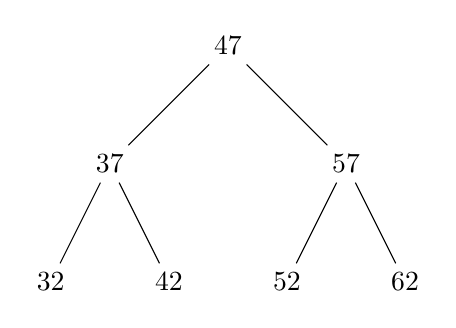
\begin{tikzpicture}[level distance=1.5cm,
  level 1/.style={sibling distance=3cm},
  level 2/.style={sibling distance=1.5cm}]
  \node {47}
    child {node {37}
      child {node {32}}
      child {node {42}}
    }
    child {node {57}
      child {node {52}}
      child {node {62}}
    };
\end{tikzpicture}
\caption{Пример бинарного дерева поиска}
\end{figure}

\item Написать программу на Python, которая реализует бинарное дерево поиска с инкапсуляцией. Программа должна создавать экземпляры класса DistrictNode, которые представляют узлы дерева, и класса AreaTree, который представляет дерево поиска. Класс AreaTree должен содержать методы для вставки, поиска и удаления элементов, при этом все рекурсивные методы должны быть приватными. Программа также должна создавать дерево поиска, вставлять в него случайные числа и выполнять поиск элементов в дереве.

Инструкции:
\begin{enumerate}
    \item Создайте класс DistrictNode с методом \_\_init\_\_, который принимает параметр district\_value и сохраняет его в атрибуте self.tree\_area. Атрибуты self.left\_sector и self.right\_sector должны быть инициализированы как None.
    \item Создайте класс AreaTree с методом \_\_init\_\_, который инициализирует атрибут self.start\_area как None.
    \item Создайте публичный метод insert\_sector в классе AreaTree, который вставляет значение в дерево. Если self.start\_area отсутствует, создайте новый узел с вставляемым значением. В противном случае, вызовите приватный метод \_insert\_sector\_helper, передав ему self.start\_area и значение.
    \item Создайте приватный метод \_insert\_sector\_helper в классе AreaTree, который рекурсивно вставляет значение в дерево. Если значение меньше или равно значению текущего узла, вставьте его в левое поддерево. Если значение строго больше значения текущего узла, вставьте его в правое поддерево.
    \item Создайте публичный метод search\_sector в классе AreaTree, который ищет значение в дереве. Если дерево пустое, верните None. В противном случае, вызовите приватный метод \_search\_sector\_rec, передав ему self.start\_area и искомое значение.
    \item Создайте приватный метод \_search\_sector\_rec в классе AreaTree, который рекурсивно ищет значение в дереве. Если текущий узел равен None или значение текущего узла равно искомому значению, верните текущий узел. В противном случае, рекурсивно вызывайте метод \_search\_sector\_rec для поиска значения в левом поддереве (если искомое значение меньше или равно текущему) или в правом поддереве (если искомое значение больше).
    \item Создайте экземпляр класса AreaTree и вставьте в него 45 случайных чисел от 25 до 65.
    \item Выполните поиск элементов в дереве и выведите результаты на экран.
\end{enumerate}

Пример использования:
\begin{lstlisting}[language=Python]
at = AreaTree()
for i in range(45):
    at.insert_sector(random.randint(25, 65))

print("Поиск элементов:")
print(at.search_sector(38))  # Обнаружено, возвращен узел (38)
print(at.search_sector(78))  # Не обнаружено, возвращено None
print(at.search_sector(58))  # Обнаружено, возвращен узел (58)
\end{lstlisting}

\begin{figure}[h]
\centering
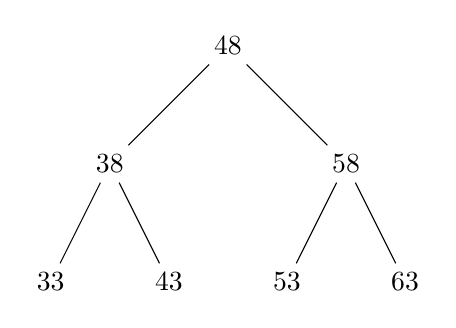
\begin{tikzpicture}[level distance=1.5cm,
  level 1/.style={sibling distance=3cm},
  level 2/.style={sibling distance=1.5cm}]
  \node {48}
    child {node {38}
      child {node {33}}
      child {node {43}}
    }
    child {node {58}
      child {node {53}}
      child {node {63}}
    };
\end{tikzpicture}
\caption{Пример бинарного дерева поиска}
\end{figure}

\item Написать программу на Python, которая реализует бинарное дерево поиска с инкапсуляцией. Программа должна создавать экземпляры класса SectorNode, которые представляют узлы дерева, и класса DistrictStructure, который представляет дерево поиска. Класс DistrictStructure должен содержать методы для вставки, поиска и удаления элементов, при этом все вспомогательные методы должны быть приватными. Программа также должна создавать дерево поиска, вставлять в него случайные числа и выполнять поиск элементов в дереве.

Инструкции:
\begin{enumerate}
    \item Создайте класс SectorNode с методом \_\_init\_\_, который принимает параметр sector\_val и сохраняет его в атрибуте self.structure\_district. Атрибуты self.left\_block и self.right\_block должны быть инициализированы как None.
    \item Создайте класс DistrictStructure с методом \_\_init\_\_, который инициализирует атрибут self.top\_district как None.
    \item Создайте публичный метод add\_block в классе DistrictStructure, который вставляет значение в дерево. Если self.top\_district отсутствует, создайте новый узел с вставляемым значением. В противном случае, вызовите приватный метод \_add\_block\_rec, передав ему self.top\_district и значение.
    \item Создайте приватный метод \_add\_block\_rec в классе DistrictStructure, который рекурсивно вставляет значение в дерево. Если значение строго меньше значения текущего узла, вставьте его в левое поддерево. Если значение больше или равно значению текущего узла, вставьте его в правое поддерево.
    \item Создайте публичный метод locate\_block в классе DistrictStructure, который ищет значение в дереве. Если дерево пустое, верните None. В противном случае, вызовите приватный метод \_locate\_block\_helper, передав ему self.top\_district и искомое значение.
    \item Создайте приватный метод \_locate\_block\_helper в классе DistrictStructure, который рекурсивно ищет значение в дереве. Если текущий узел равен None или значение текущего узла равно искомому значению, верните текущий узел. В противном случае, рекурсивно вызывайте метод \_locate\_block\_helper для поиска значения в левом поддереве (если искомое значение меньше текущего) или в правом поддереве (если искомое значение больше или равно текущему).
    \item Создайте экземпляр класса DistrictStructure и вставьте в него 46 случайных чисел от 26 до 66.
    \item Выполните поиск элементов в дереве и выведите результаты на экран.
\end{enumerate}

Пример использования:
\begin{lstlisting}[language=Python]
ds = DistrictStructure()
for i in range(46):
    ds.add_block(random.randint(26, 66))

print("Поиск элементов:")
print(ds.locate_block(39))  # Обнаружено, возвращен узел (39)
print(ds.locate_block(79))  # Не обнаружено, возвращено None
print(ds.locate_block(59))  # Обнаружено, возвращен узел (59)
\end{lstlisting}

\begin{figure}[h]
\centering
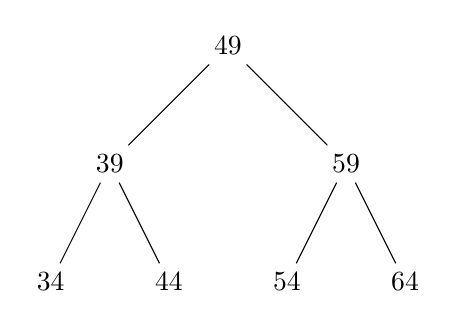
\begin{tikzpicture}[level distance=1.5cm,
  level 1/.style={sibling distance=3cm},
  level 2/.style={sibling distance=1.5cm}]
  \node {49}
    child {node {39}
      child {node {34}}
      child {node {44}}
    }
    child {node {59}
      child {node {54}}
      child {node {64}}
    };
\end{tikzpicture}
\caption{Пример бинарного дерева поиска}
\end{figure}

\item Написать программу на Python, которая реализует бинарное дерево поиска с инкапсуляцией. Программа должна создавать экземпляры класса BlockNode, которые представляют узлы дерева, и класса SectorIndex, который представляет дерево поиска. Класс SectorIndex должен содержать методы для вставки, поиска и удаления элементов, при этом все рекурсивные методы должны быть приватными. Программа также должна создавать дерево поиска, вставлять в него случайные числа и выполнять поиск элементов в дереве.

Инструкции:
\begin{enumerate}
    \item Создайте класс BlockNode с методом \_\_init\_\_, который принимает параметр block\_value и сохраняет его в атрибуте self.index\_sector. Атрибуты self.left\_unit и self.right\_unit должны быть инициализированы как None.
    \item Создайте класс SectorIndex с методом \_\_init\_\_, который инициализирует атрибут self.root\_sector как None.
    \item Создайте публичный метод insert\_unit в классе SectorIndex, который вставляет значение в дерево. Если self.root\_sector отсутствует, создайте новый узел с вставляемым значением. В противном случае, вызовите приватный метод \_insert\_unit\_helper, передав ему self.root\_sector и значение.
    \item Создайте приватный метод \_insert\_unit\_helper в классе SectorIndex, который рекурсивно вставляет значение в дерево. Если значение меньше или равно значению текущего узла, вставьте его в левое поддерево. Если значение строго больше значения текущего узла, вставьте его в правое поддерево.
    \item Создайте публичный метод find\_unit в классе SectorIndex, который ищет значение в дереве. Если дерево пустое, верните None. В противном случае, вызовите приватный метод \_find\_unit\_rec, передав ему self.root\_sector и искомое значение.
    \item Создайте приватный метод \_find\_unit\_rec в классе SectorIndex, который рекурсивно ищет значение в дереве. Если текущий узел равен None или значение текущего узла равно искомому значению, верните текущий узел. В противном случае, рекурсивно вызывайте метод \_find\_unit\_rec для поиска значения в левом поддереве (если искомое значение меньше или равно текущему) или в правом поддереве (если искомое значение больше).
    \item Создайте экземпляр класса SectorIndex и вставьте в него 47 случайных чисел от 27 до 67.
    \item Выполните поиск элементов в дереве и выведите результаты на экран.
\end{enumerate}

Пример использования:
\begin{lstlisting}[language=Python]
si = SectorIndex()
for i in range(47):
    si.insert_unit(random.randint(27, 67))

print("Поиск элементов:")
print(si.find_unit(40))  # Обнаружено, возвращен узел (40)
print(si.find_unit(80))  # Не обнаружено, возвращено None
print(si.find_unit(60))  # Обнаружено, возвращен узел (60)
\end{lstlisting}

\begin{figure}[h]
\centering
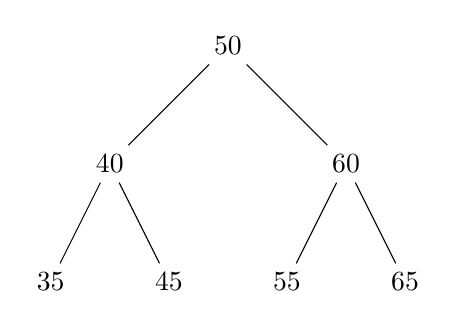
\begin{tikzpicture}[level distance=1.5cm,
  level 1/.style={sibling distance=3cm},
  level 2/.style={sibling distance=1.5cm}]
  \node {50}
    child {node {40}
      child {node {35}}
      child {node {45}}
    }
    child {node {60}
      child {node {55}}
      child {node {65}}
    };
\end{tikzpicture}
\caption{Пример бинарного дерева поиска}
\end{figure}

\end{enumerate}